% Diapositives de la partie théorique du cours « Introduction à AWS »
% Compilation : latexmk -lualatex main.tex
\documentclass[aspectratio=169,11pt]{beamer}
% =====================================================================
%  Thème des diapositives « Introduction à AWS »
%  Support de formation : un module par séance, sommaire rappelé à chaque
%  module, diapos de TP et de questions, numérotation « module - page ».
%  Figures : ../static/figures (TikZ + icônes officielles AWS).
% =====================================================================
\usepackage{fontspec}
\setsansfont{Inter}[Scale=0.95]
\setmonofont{DejaVu Sans Mono}[Scale=0.78]
\usefonttheme{professionalfonts}
\usepackage[french]{babel}
\usepackage{tikz}
\usetikzlibrary{positioning,calc,arrows.meta,fit}
\usepackage{tcolorbox}
\usepackage{booktabs}
\usepackage{tabularx}
\usepackage{array}
\usepackage{colortbl}
\usepackage{listings}
\usepackage{fontawesome5}
\graphicspath{{../static/figures/}{../figures/icones/}}
\hyphenpenalty=10000
\exhyphenpenalty=10000

% ---- couleurs --------------------------------------------------------
\definecolor{Squid}{HTML}{232F3E}
\definecolor{Orange}{HTML}{EC7211}
\definecolor{Encre}{HTML}{16191F}
\definecolor{Gris}{HTML}{5F6B7A}
\definecolor{Ligne}{HTML}{D1D5DB}
\definecolor{Doux}{HTML}{F2F3F3}
\definecolor{Lien}{HTML}{0972D3}
\definecolor{Rouge}{HTML}{D91515}
\definecolor{Vert}{HTML}{037F0C}

\hypersetup{colorlinks=true, urlcolor=Lien, linkcolor=Squid}
\setbeamercolor{normal text}{fg=Encre}
\setbeamercolor{structure}{fg=Squid}
\setbeamercolor{alerted text}{fg=Orange}
\setbeamercolor{item}{fg=Squid}
\setbeamertemplate{navigation symbols}{}
\setbeamertemplate{itemize item}{\raisebox{.18em}{\color{Squid}\rule{.36em}{.36em}}}
\setbeamertemplate{itemize subitem}{\raisebox{.22em}{\color{Gris}\rule{.26em}{.26em}}}
\setbeamertemplate{enumerate item}{\color{Squid}\bfseries\insertenumlabel.}
\setlength{\leftmargini}{1.1em}
\setlength{\leftmarginii}{1.1em}
\setbeamerfont{itemize/enumerate subbody}{size=\normalsize}

% ---- numérotation « module - page » ------------------------------------
\newcount\debutmodule \debutmodule=0
\newcommand{\numdiapo}{%
  \ifnum\value{section}>0 \thesection\,-\,\the\numexpr\value{framenumber}-\debutmodule\relax
  \else\insertframenumber\fi}

% ---- titre de diapo : capitales, bandeau orange, module en haut à droite --
\setbeamertemplate{frametitle}{%
  \vspace*{.7em}%
  {\usebeamerfont{frametitle}\Large\bfseries\color{Squid}\MakeUppercase{\insertframetitle}}\par
  \vspace*{-.1em}}
\setbeamertemplate{headline}{%
  \begin{tikzpicture}[remember picture, overlay]
    \fill[Orange] (current page.north west) rectangle ([yshift=-.11cm]current page.north east);
  \end{tikzpicture}}
\setbeamertemplate{footline}{%
  \begin{tikzpicture}[remember picture, overlay]
    \node[anchor=west, font=\scriptsize, text=Gris] at ([xshift=.6cm,yshift=.35cm]current page.south west) {\textbf{\numdiapo}\quad Introduction à AWS};
    \ifnum\value{section}>0
      \node[anchor=east, font=\scriptsize, text=Gris] at ([xshift=-.6cm,yshift=.35cm]current page.south east) {Module \thesection\ · \insertsectionhead};
    \fi
  \end{tikzpicture}}

% ---- source et lien vers la documentation ----------------------------------
\newcommand{\source}[1]{%
  \begin{tikzpicture}[remember picture, overlay]
    \node[anchor=south west, font=\tiny, text=Gris, text width=13.6cm, align=left, inner sep=0pt]
      at ([xshift=.6cm,yshift=.72cm]current page.south west) {Source : #1};
  \end{tikzpicture}}
\newtcolorbox{encadrelien}{colback=Doux, colframe=Doux, sharp corners, boxrule=0pt,
  left=6pt, right=6pt, top=3pt, bottom=3pt, fontupper=\small}
\newcommand{\lien}[1]{\begin{encadrelien}\url{#1}\end{encadrelien}}

% ---- mise en garde en ligne --------------------------------------------------
\newcommand{\attention}{{\color{Orange}\faExclamationTriangle}\ }

% ---- terminal pour une commande ---------------------------------------------
\newtcolorbox{terminal}{colback=Squid, colframe=Squid, sharp corners, boxrule=0pt,
  left=8pt, right=8pt, top=4pt, bottom=4pt, fontupper=\ttfamily\small\color{white}}

% ---- JSON ---------------------------------------------------------------------
\lstdefinelanguage{json}{morestring=[b]", stringstyle=\color{Lien}, literate={:}{{\color{Gris}:}}1}
\lstset{basicstyle=\ttfamily\footnotesize, columns=fullflexible, keepspaces=true,
  backgroundcolor=\color{Doux}, frame=none, xleftmargin=6pt, xrightmargin=6pt,
  aboveskip=4pt, belowskip=4pt, showstringspaces=false, upquote=true,
  literate={é}{{\'e}}1 {è}{{\`e}}1 {à}{{\`a}}1}

% ---- flèche des schémas propres aux diapos ---------------------------------------
\tikzset{fl/.style={-{Stealth[length=2.4mm]}, line width=1pt, draw=#1}, fl/.default=Encre}

% ---- liste des modules (sommaire) ------------------------------------------------
\newcommand{\listemodules}{%
  {Introduction à AWS},
  {Sécurité et gestion des accès},
  {Calcul : Amazon EC2},
  {Stockage, bases de données et messages},
  {Projet final}}
\newcommand{\sommaire}[1]{%
  \begin{frame}{Sommaire}
    \begin{tikzpicture}[x=1cm,y=1cm]
      \foreach \titre [count=\n] in \listemodules {
        \ifnum\n=#1
          \node[anchor=west, font=\large\bfseries, text=Orange] at (0,-\n*.82) {\n.\enspace\titre};
          \fill[Orange] (-.35,-\n*.82-.2) rectangle ++(.1,.4);
        \else
          \node[anchor=west, font=\large, text=Gris] at (0,-\n*.82) {\n.\enspace\titre};
        \fi
      }
    \end{tikzpicture}
  \end{frame}}

% ---- page de module (à chaque \section) --------------------------------------------
\AtBeginSection{%
  \global\debutmodule=\numexpr\value{framenumber}\relax
  {\setbeamertemplate{headline}{\begin{tikzpicture}[remember picture, overlay]\fill[Orange] (current page.north west) rectangle ([yshift=-.11cm]current page.north east);\end{tikzpicture}}
   \begin{frame}[plain]
     \begin{tikzpicture}[remember picture, overlay]
       \fill[Orange] (current page.north west) rectangle ([yshift=-.11cm]current page.north east);
       \node[circle, fill=Squid, text=white, font=\fontsize{30}{30}\selectfont\bfseries, minimum size=2.2cm] at ([yshift=1.1cm]current page.center) {\thesection};
       \node[font=\fontsize{24}{28}\selectfont\bfseries, text=Squid, text width=13cm, align=center] at ([yshift=-.9cm]current page.center) {\MakeUppercase{\insertsectionhead}};
     \end{tikzpicture}
   \end{frame}}
  \sommaire{\value{section}}}

% ---- diapo de TP -----------------------------------------------------------------
\newcommand{\diapotp}[3]{% numéro, titre, éléments \item
  \begin{frame}[plain]
    \begin{tikzpicture}[remember picture, overlay]
      \fill[Orange] (current page.north west) rectangle ([yshift=-.11cm]current page.north east);
      \fill[Squid] (current page.north west) rectangle ([xshift=5.2cm]current page.south west);
      \node[font=\fontsize{40}{40}\selectfont\bfseries, text=white] at ([xshift=2.6cm,yshift=.5cm]current page.west) {TP #1};
      \node[font=\large, text=Ligne, text width=4.2cm, align=center] at ([xshift=2.6cm,yshift=-.7cm]current page.west) {#2};
      \node[anchor=west, text width=8.6cm] at ([xshift=6.1cm]current page.west) {%
        \begin{minipage}{8.6cm}\begin{itemize}\setlength{\itemsep}{.6em}#3\end{itemize}\end{minipage}};
    \end{tikzpicture}
  \end{frame}}

% ---- icône de service avec légende -------------------------------------------------------
\newcommand{\service}[3][1.2cm]{%
  \begin{tabular}{@{}c@{}}\includegraphics[width=#1]{#2}\\[.15em]\parbox[t]{2.7cm}{\centering\small #3}\end{tabular}}


\begin{document}

% ---- page de titre ------------------------------------------------------
\begin{frame}[plain]
  \begin{tikzpicture}[remember picture, overlay]
    \fill[Orange] (current page.north west) rectangle ([yshift=-.11cm]current page.north east);
    \fill[Squid] ([yshift=-2.3cm]current page.west) rectangle ([yshift=2.3cm]current page.east);
    \node[anchor=west, font=\fontsize{36}{40}\selectfont\bfseries, text=white] at ([xshift=1.2cm,yshift=.55cm]current page.west) {INTRODUCTION À AWS};
    \node[anchor=west, font=\LARGE, text=Ligne] at ([xshift=1.2cm,yshift=-.55cm]current page.west) {IAM, EC2, S3, SQS et un projet de déploiement};
    \node[anchor=west, font=\large, text=Gris] at ([xshift=1.2cm,yshift=-3.1cm]current page.west) {Romial Menra};
  \end{tikzpicture}
\end{frame}

\sommaire{0}

\begin{frame}{Organisation}
  \begin{itemize}
    \setlength{\itemsep}{.6em}
    \item 5 modules, chacun suivi d'un TP sur la console AWS
    \item Compte AWS fourni : un utilisateur IAM par étudiant
    \item Région de travail : \texttt{eu-west-3} (Paris)
    \item Fil conducteur : une application web publique sur EC2, qui stocke ses fichiers dans S3
  \end{itemize}
  \bigskip
  \begin{itemize}
    \item Support de cours et énoncés des TP : site du cours
    \item Documentation de référence :
  \end{itemize}
  \lien{https://docs.aws.amazon.com}
\end{frame}

% =====================================================================
%  Module 1 : Introduction à AWS
% =====================================================================
\section{Introduction à AWS}

\begin{frame}{Amazon Web Services}
  \begin{itemize}
    \setlength{\itemsep}{.55em}
    \item Filiale cloud d'Amazon, lancée en 2006
    \item Infrastructure et services informatiques à la demande, accessibles par API
    \item Premier fournisseur mondial de cloud : 28 \% du marché (T2 2026)
    \item Chiffre d'affaires 2025 : 128,7 milliards de dollars (+20 \% sur un an)
  \end{itemize}
  \bigskip
  \textbf{Principes fondateurs}
  \begin{itemize}
    \item API d'abord : tout se pilote par programme
    \item Libre-service : ressources disponibles en quelques minutes, sans intervention humaine
    \item Paiement à l'usage : à la seconde, au gigaoctet, à la requête
  \end{itemize}
  \source{Amazon, \emph{Fourth Quarter 2025 Results} ; Synergy Research Group, Q2 2026.}
\end{frame}

\begin{frame}{Quelques dates}
  \renewcommand{\arraystretch}{1.3}
  \begin{tabular}{@{}l l@{}}
    \textbf{2002} & premiers services web d'Amazon pour les développeurs \\
    \textbf{2006} & S3 (mars), SQS (juillet), EC2 (août) : les trois services d'origine \\
    \textbf{2009} & VPC et RDS \\
    \textbf{2012} & DynamoDB \\
    \textbf{2014} & Lambda (fonctions serverless) \\
    \textbf{2017} & ouverture de la région de Paris (\texttt{eu-west-3}) \\
    \textbf{2026} & 39 régions, 123 zones de disponibilité, plus de 1 200 types d'instances EC2 \\
  \end{tabular}
  \source{AWS News Blog, « Twenty years of Amazon S3 », « Happy 20th Birthday, Amazon EC2 », « Amazon SQS turns 20 », 2026.}
\end{frame}

\begin{frame}{Parts de marché du cloud (T2 2026)}
  \begin{columns}[c]
    \begin{column}{.55\textwidth}
      \begin{tikzpicture}[x=1cm,y=1cm]
        \foreach \nom/\part/\coul [count=\i from 0] in {AWS/28/Orange, Microsoft Azure/20/Lien, Google Cloud/15/Vert, Autres/37/Ligne}{
          \node[anchor=east, font=\small] at (0,-\i*.9) {\nom};
          \fill[\coul] (.15,-\i*.9-.28) rectangle ++(\part*.1,.56);
          \node[anchor=west, font=\small\bfseries] at (\part*.1+.25,-\i*.9) {\part\ \%};
        }
      \end{tikzpicture}
    \end{column}
    \begin{column}{.42\textwidth}
      \begin{itemize}
        \setlength{\itemsep}{.5em}
        \item Marché mondial de l'infrastructure cloud : 143,4 Md\$ sur le trimestre
        \item Croissance d'environ 43 \% sur un an
        \item Les trois premiers : 63 \% du marché
      \end{itemize}
    \end{column}
  \end{columns}
  \source{Synergy Research Group, « Cloud Market Share Trends », Q2 2026.}
\end{frame}

\begin{frame}{Modèles de service}
  \renewcommand{\arraystretch}{1.45}
  \begin{tabularx}{\textwidth}{@{}l>{\raggedright\arraybackslash}X>{\raggedright\arraybackslash}X@{}}
    \toprule
    & \textbf{Le client gère} & \textbf{Exemples AWS} \\ \midrule
    \textbf{IaaS} & système d'exploitation, logiciels, données, accès & EC2, EBS, VPC \\
    \textbf{PaaS} & code, données, accès & RDS, Lambda, Elastic Beanstalk \\
    \textbf{SaaS} & données, accès & Amazon WorkMail, Amazon Connect \\ \bottomrule
  \end{tabularx}
  \bigskip
  \begin{itemize}
    \item Plus le service est géré, moins il y a d'administration, et moins de contrôle
    \item Les données et les droits d'accès restent toujours à la charge du client
  \end{itemize}
\end{frame}

\begin{frame}{Modèle de responsabilité partagée}
  \begin{columns}[c]
    \begin{column}{.6\textwidth}
      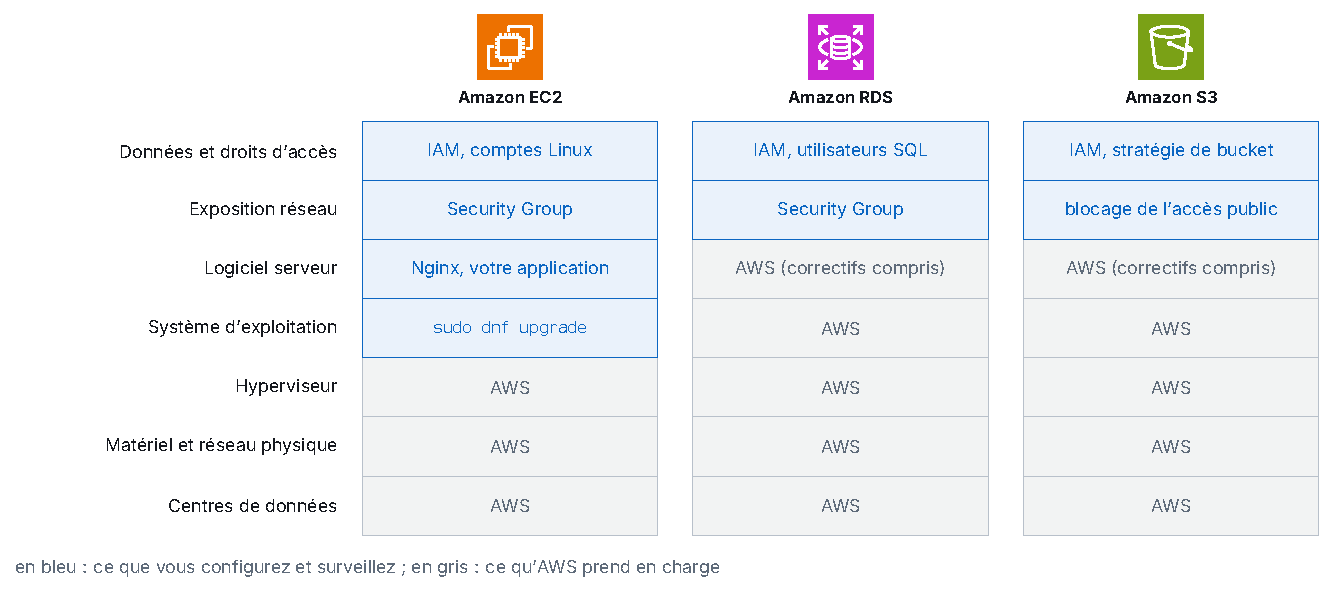
\includegraphics[width=\textwidth]{responsabilite}
    \end{column}
    \begin{column}{.38\textwidth}
      \begin{itemize}
        \setlength{\itemsep}{.6em}
        \item AWS : sécurité \textbf{du} cloud (bâtiments, matériel, réseau, virtualisation)
        \item Client : sécurité \textbf{dans} le cloud (configuration, mises à jour, données, IAM)
        \item La frontière dépend du service
      \end{itemize}
    \end{column}
  \end{columns}
  \lien{https://aws.amazon.com/compliance/shared-responsibility-model/}
\end{frame}

\begin{frame}{Catalogue de services}
  \centering
  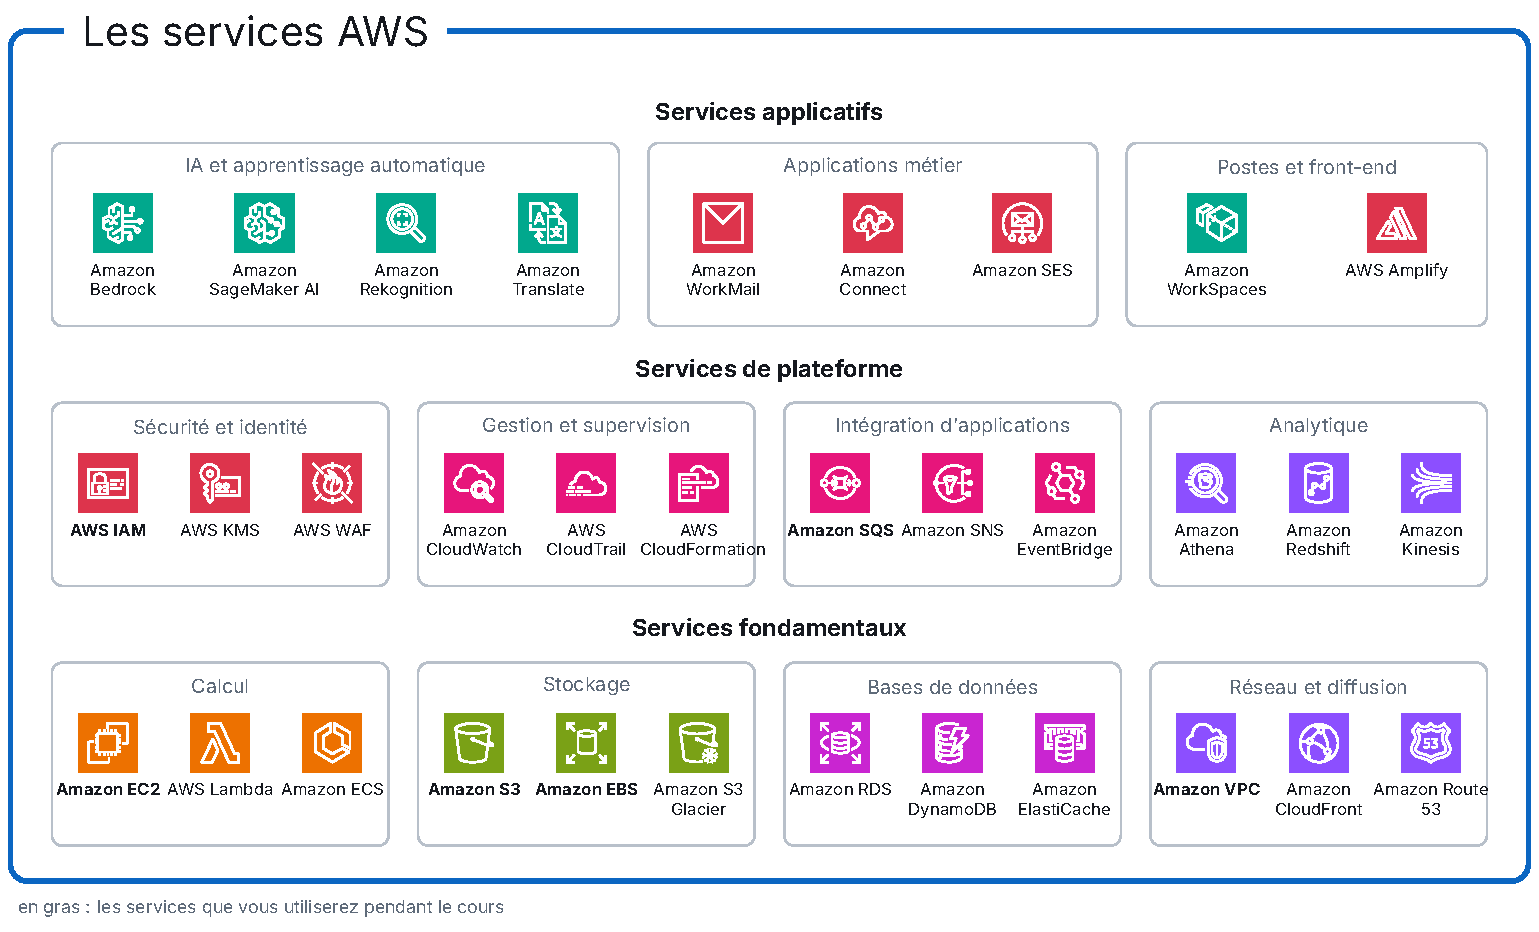
\includegraphics[height=.74\textheight]{familles-services}
  \source{AWS, \emph{Overview of Amazon Web Services} : plus de 200 services.}
\end{frame}

\begin{frame}{Infrastructure classique et équivalents AWS}
  \centering
  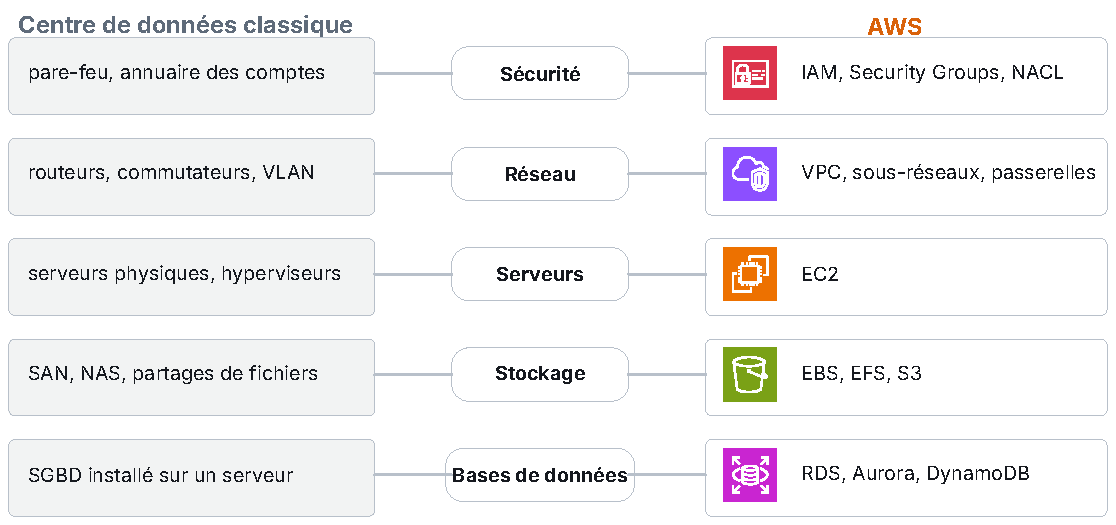
\includegraphics[width=.92\textwidth]{infra-correspondance}
\end{frame}

\begin{frame}{Infrastructure mondiale : régions}
  \begin{itemize}
    \setlength{\itemsep}{.55em}
    \item Région : zone géographique regroupant plusieurs zones de disponibilité
    \item 39 régions en 2026, d'autres annoncées
    \item Régions indépendantes : une panne reste en principe confinée à sa région
    \item Les données restent dans la région choisie, sauf réplication explicite
    \item Chaque région a un code : \texttt{eu-west-3} (Paris), \texttt{eu-central-1} (Francfort), \texttt{us-east-1} (Virginie du Nord)
    \item Certaines régions récentes doivent être activées (\emph{opt-in}) : \texttt{af-south-1}, \texttt{eu-south-1}...
  \end{itemize}
  \lien{https://aws.amazon.com/about-aws/global-infrastructure/regions_az/}
\end{frame}

\begin{frame}{Régions, zones de disponibilité, points de présence}
  \centering
  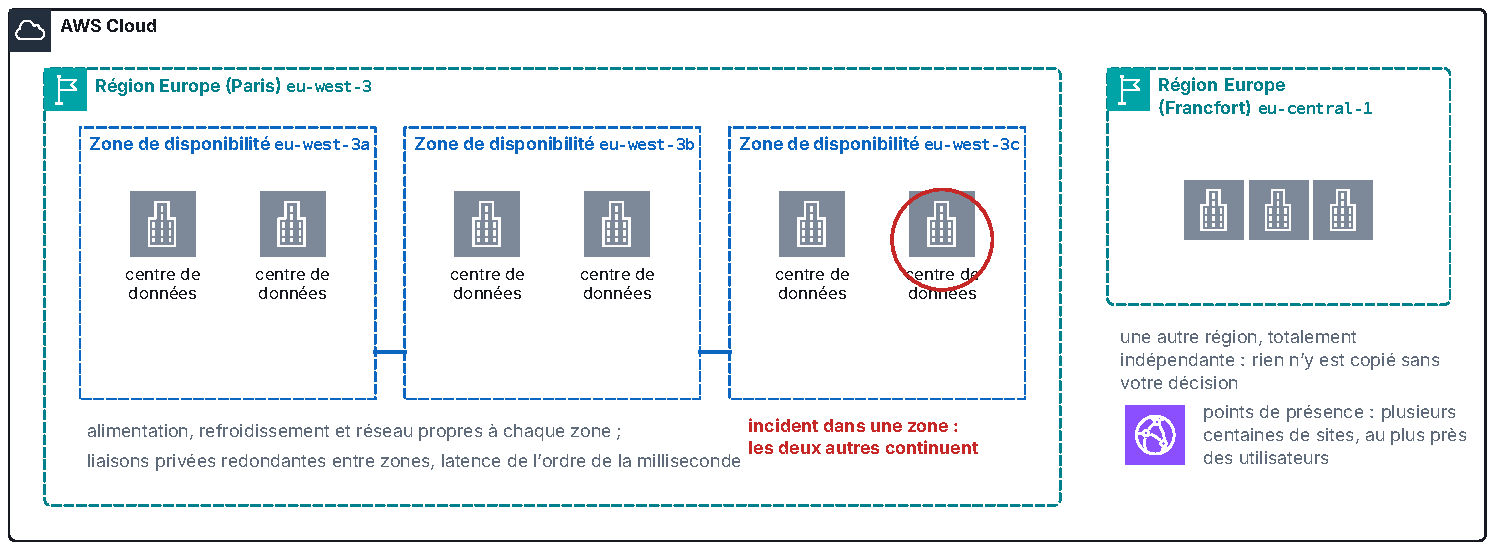
\includegraphics[width=\textwidth]{region-az}
\end{frame}

\begin{frame}{Zones de disponibilité (AZ)}
  \begin{itemize}
    \setlength{\itemsep}{.55em}
    \item Un ou plusieurs centres de données à l'intérieur d'une région
    \item Alimentation, refroidissement et réseau propres
    \item Distantes les unes des autres, mais à moins de 100 km : latence de l'ordre de la milliseconde
    \item Paris : 3 AZ, \texttt{eu-west-3a}, \texttt{eu-west-3b}, \texttt{eu-west-3c}
    \item Points de présence : plusieurs centaines de sites pour CloudFront et Route 53
  \end{itemize}
  \bigskip
  \attention Un sous-réseau, un volume EBS et une instance EC2 vivent dans \textbf{une seule} AZ
\end{frame}

\begin{frame}{Haute disponibilité}
  \centering
  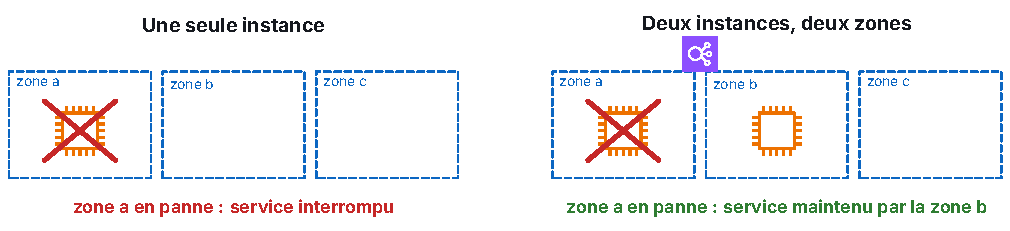
\includegraphics[width=.9\textwidth]{haute-dispo}\par\bigskip
  \raggedright
  \begin{itemize}
    \item Haute disponibilité = ressources réparties sur au moins deux AZ
    \item Pour EC2 : plusieurs instances derrière un répartiteur de charge (ELB)
    \item Pour une base RDS : déploiement Multi-AZ (copie de secours synchrone)
  \end{itemize}
\end{frame}

\begin{frame}{Services et régions}
  \begin{itemize}
    \setlength{\itemsep}{.55em}
    \item Tous les services ne sont pas disponibles dans toutes les régions
    \item Les nouveautés arrivent souvent d'abord en \texttt{us-east-1}
    \item Les prix varient d'une région à l'autre
    \item Services \textbf{régionaux} : EC2, EBS, VPC, RDS, SQS... (la console affiche une région)
    \item Services \textbf{globaux} : IAM, Route 53, CloudFront (la console affiche « Global »)
    \item S3 : liste des buckets globale, mais chaque bucket appartient à une région
  \end{itemize}
  \bigskip
  \attention Une ressource créée dans une autre région n'apparaît pas dans la console
  \lien{https://aws.amazon.com/about-aws/global-infrastructure/regional-product-services/}
\end{frame}

\begin{frame}{Choisir une région}
  \begin{enumerate}
    \setlength{\itemsep}{.6em}
    \item \textbf{Réglementation} : localisation des données (RGPD, données de santé, secteur public)
    \item \textbf{Latence} : proximité des utilisateurs, à mesurer
    \item \textbf{Services disponibles} dans la région
    \item \textbf{Prix}
  \end{enumerate}
  \bigskip
  Pour ce cours : \texttt{eu-west-3} (Paris), ouverte en décembre 2017, 3 AZ
\end{frame}

\begin{frame}{Idée reçue n°1 : « le cloud n'est pas fiable »}
  \begin{itemize}
    \setlength{\itemsep}{.5em}
    \item Engagements de service (SLA) publiés pour chaque service
    \begin{itemize}
      \item EC2 : 99,99 \% par mois pour un déploiement sur plusieurs AZ, 99,5 \% pour une instance seule
      \item S3 Standard : 99,9 \% de disponibilité, durabilité conçue pour 99,999999999 \% (11 neuf)
    \end{itemize}
    \item Données S3 copiées dans plusieurs AZ
  \end{itemize}
  \bigskip
  \attention Les pannes existent :
  \begin{itemize}
    \item 28/02/2017 : S3 indisponible plus de 4 h en \texttt{us-east-1} (erreur de commande)
    \item 19-20/10/2025 : panne de DynamoDB d'environ 14 h en \texttt{us-east-1}, avec effet en cascade sur EC2, Lambda, STS...
  \end{itemize}
  \source{AWS, \emph{Amazon Compute SLA}, \emph{Amazon S3 SLA} ; AWS, résumés des incidents du 28/02/2017 et du 19-20/10/2025.}
\end{frame}

\begin{frame}{Idée reçue n°2 : « je perds le contrôle de mes données »}
  \begin{itemize}
    \setlength{\itemsep}{.6em}
    \item Le client reste propriétaire de ses données
    \item Il choisit la région où elles sont stockées
    \item Chiffrement au repos et en transit, avec des clés gérées par AWS ou par le client (KMS)
    \item Récupération des données à tout moment (API, transfert, AWS Snowball)
    \item Journal de tous les appels d'API du compte (CloudTrail)
  \end{itemize}
\end{frame}

\begin{frame}{Tarification}
  \begin{itemize}
    \setlength{\itemsep}{.5em}
    \item Paiement à l'usage, facture mensuelle
    \item Chaque service a ses propres unités : heure ou seconde, Go-mois, requêtes, Go transférés
    \item Coût difficile à prévoir sans estimation préalable
    \item Pas d'arrêt automatique en cas de dépassement : un budget AWS envoie une alerte, il ne coupe rien
    \item Comptes créés depuis le 15/07/2025 : jusqu'à 200 \$ de crédits, plan gratuit de 6 mois
    \item Transfert entrant gratuit, transfert sortant vers Internet facturé
  \end{itemize}
  \lien{https://calculator.aws}
\end{frame}

\begin{frame}{Ce qui coûte, même sans être utilisé}
  \renewcommand{\arraystretch}{1.3}
  \begin{tabularx}{\textwidth}{@{}>{\raggedright\arraybackslash}p{4.4cm}>{\raggedright\arraybackslash}X>{\raggedright\arraybackslash}p{3.8cm}@{}}
    \toprule
    \textbf{Ressource} & \textbf{Unité facturée} & \textbf{Facturée à l'arrêt ?} \\ \midrule
    Instance EC2 démarrée & seconde (minimum 60 s) & \textcolor{Rouge}{oui} \\
    Instance EC2 arrêtée & aucune pour le calcul & \textcolor{Rouge}{disque EBS facturé} \\
    Volume EBS & Go provisionné par mois & \textcolor{Rouge}{oui} \\
    Adresse IPv4 publique & heure (0,005 \$) depuis 02/2024 & \textcolor{Rouge}{oui} \\
    NAT Gateway & heure + Go traité & \textcolor{Rouge}{oui} \\
    Objet S3 & Go-mois + requêtes & selon le volume \\ \bottomrule
  \end{tabularx}
  \source{AWS, pages de tarification ; AWS News Blog, « New – AWS Public IPv4 Address Charge », 2023.}
\end{frame}

\begin{frame}{Accès à AWS}
  \centering
  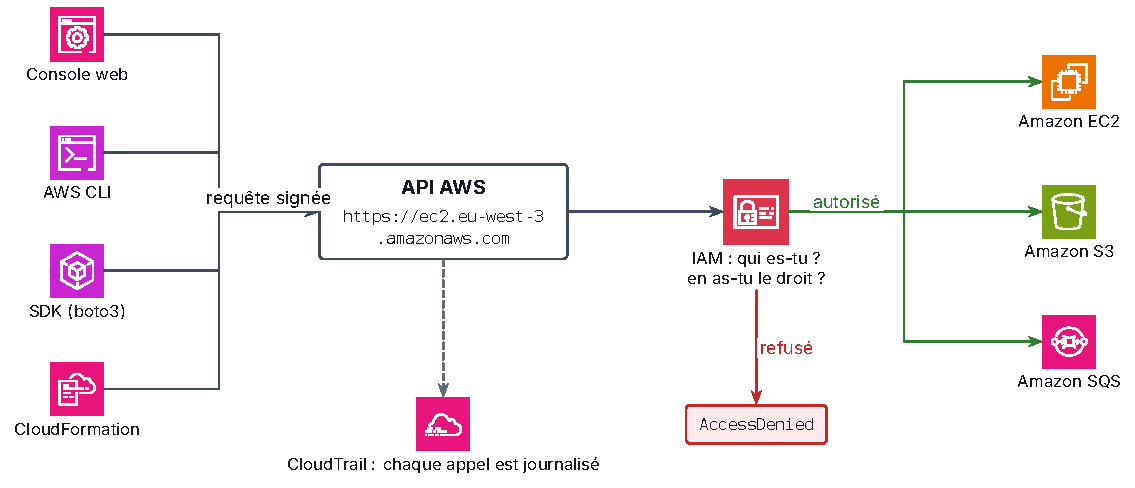
\includegraphics[height=.56\textheight]{appel-api}\par\medskip
  \raggedright
  \begin{itemize}
    \item Console web : découverte, diagnostic
    \item CLI (\texttt{aws}) et SDK (\texttt{boto3}...) : scripts et applications
    \item Infrastructure as Code : CloudFormation, CDK, Terraform, Pulumi
  \end{itemize}
\end{frame}

\begin{frame}[fragile]{AWS CLI et CloudShell}
  \begin{itemize}
    \setlength{\itemsep}{.5em}
    \item CloudShell : terminal intégré à la console, déjà authentifié, CLI installée
    \item Toute action passe par un appel d'API signé, contrôlé par IAM
    \item Même appel, que l'on passe par la console, la CLI ou un SDK
  \end{itemize}
  \begin{terminal}
aws sts get-caller-identity\\
aws ec2 describe-availability-zones --region eu-west-3 --output table
  \end{terminal}
  \lien{https://docs.aws.amazon.com/cli/latest/reference/}
\end{frame}

\diapotp{1}{Prise en main de la console}{%
  \item Connexion avec l'utilisateur IAM fourni
  \item Région par défaut : \texttt{eu-west-3}
  \item Premières commandes dans CloudShell
  \item Lecture des prix des types d'instances}


% =====================================================================
%  Module 2 : Sécurité et gestion des accès
% =====================================================================
\section{Sécurité et gestion des accès}

\begin{frame}{IAM : Identity and Access Management}
  \begin{itemize}
    \setlength{\itemsep}{.55em}
    \item Contrôle l'accès aux services et ressources AWS
    \item \textbf{Authentification} : qui envoie la requête ?
    \item \textbf{Autorisation} : cette identité a-t-elle le droit de faire cette action sur cette ressource ?
    \item S'applique à toutes les requêtes : console, CLI, SDK
    \item Service global (pas de région), gratuit
  \end{itemize}
  \lien{https://docs.aws.amazon.com/IAM/latest/UserGuide/introduction.html}
\end{frame}

\begin{frame}{Vocabulaire}
  \renewcommand{\arraystretch}{1.45}
  \begin{tabularx}{\textwidth}{@{}>{\raggedright\arraybackslash}p{3.2cm}>{\raggedright\arraybackslash}X@{}}
    \toprule
    \textbf{Principal} & entité qui envoie une requête : utilisateur racine, utilisateur IAM, rôle, service AWS \\
    \textbf{Utilisateur IAM} & identité permanente d'une personne ou d'une application ; mot de passe et/ou clés d'accès \\
    \textbf{Groupe} & ensemble d'utilisateurs qui partagent les mêmes stratégies ; ne peut pas se connecter \\
    \textbf{Rôle} & identité sans identifiants permanents, endossée temporairement \\
    \textbf{Stratégie} (\emph{policy}) & document JSON qui autorise ou interdit des actions sur des ressources \\ \bottomrule
  \end{tabularx}
\end{frame}

\begin{frame}{Utilisateur racine}
  \begin{itemize}
    \setlength{\itemsep}{.6em}
    \item Créé avec le compte, identifié par l'adresse électronique d'inscription
    \item Tous les droits, non restreignables par IAM
    \item MFA obligatoire pour tous les types de comptes depuis juin 2025
    \item À réserver aux tâches qui l'exigent (fermeture du compte, plan de support...)
    \item Pas de clé d'accès pour l'utilisateur racine
  \end{itemize}
  \bigskip
  Dans ce cours : accès par un utilisateur IAM fourni, jamais par le compte racine
  \source{AWS, « AWS IAM now enforces MFA for root users across all account types », 2025.}
\end{frame}

\begin{frame}{Utilisateurs, groupes, rôles}
  \centering
  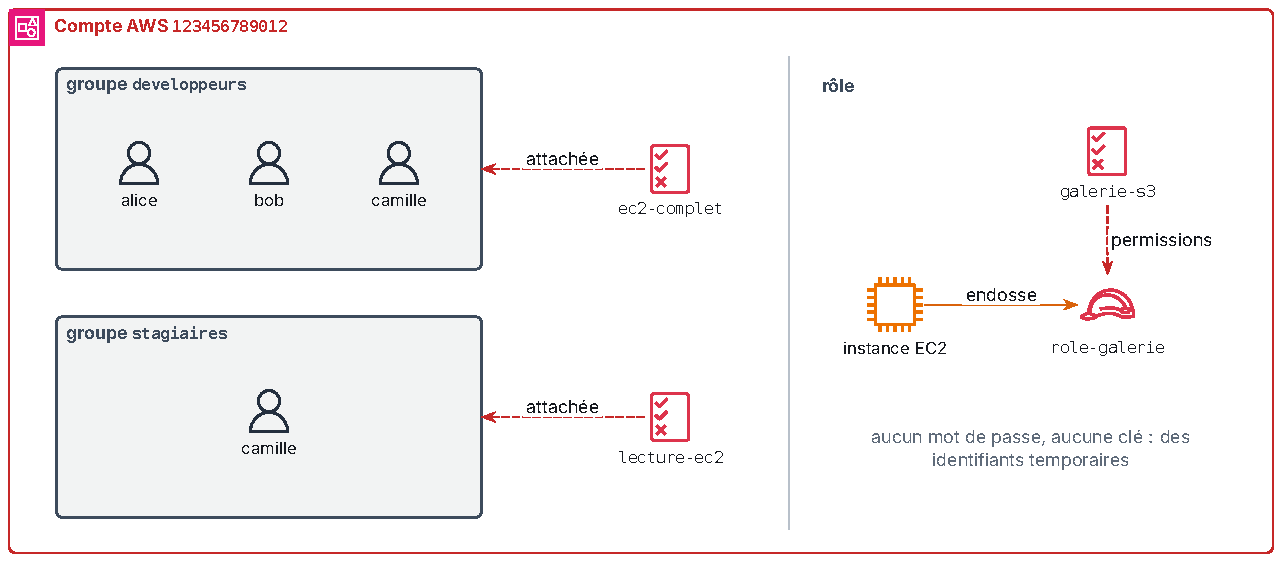
\includegraphics[width=.95\textwidth]{iam-identites}
\end{frame}

\begin{frame}{Rôles}
  \begin{itemize}
    \setlength{\itemsep}{.5em}
    \item Pas de mot de passe ni de clé permanente
    \item Endossé par une entité autorisée : service AWS (EC2, Lambda), utilisateur, autre compte, utilisateur fédéré
    \item Identifiants temporaires délivrés par AWS STS, renouvelés automatiquement
    \item Deux stratégies :
    \begin{itemize}
      \item \textbf{stratégie de confiance} : qui peut endosser le rôle
      \item \textbf{stratégie de permissions} : ce que le rôle autorise
    \end{itemize}
    \item Instance EC2 : rôle associé via un \emph{instance profile}
  \end{itemize}
  \bigskip
  \attention Une application sur AWS n'a jamais besoin de clé d'accès : elle utilise un rôle
\end{frame}

\begin{frame}{Structure d'une stratégie}
  \centering
  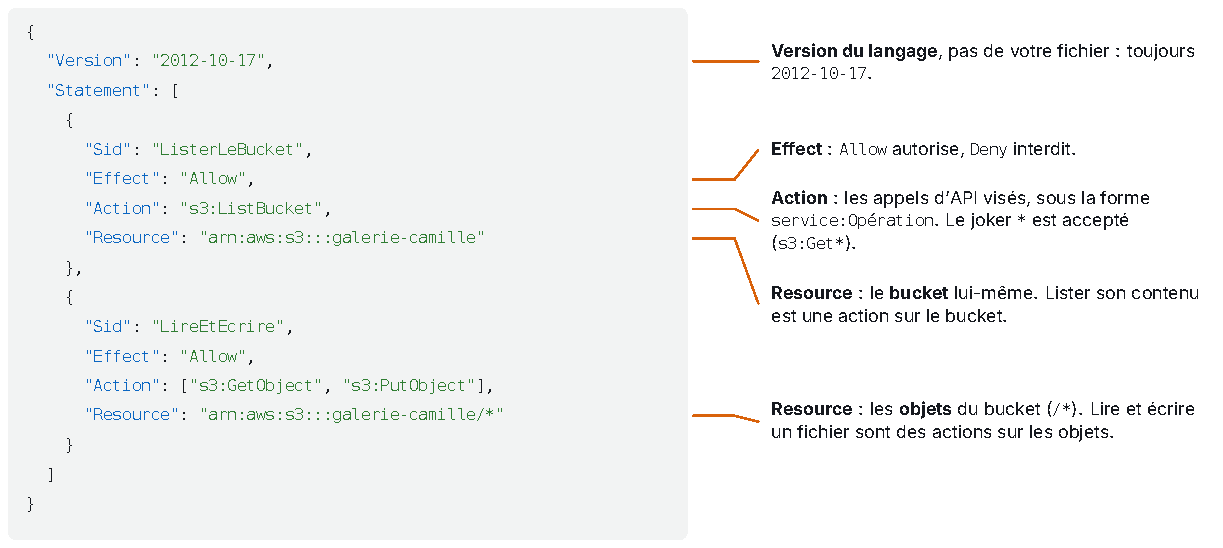
\includegraphics[width=.96\textwidth]{politique-annotee}
\end{frame}

\begin{frame}[fragile]{Stratégie avec condition}
  Exemple : interdire toute action EC2 en dehors de la région de Paris
\begin{lstlisting}[language=json]
{
  "Version": "2012-10-17",
  "Statement": [{
    "Sid": "UniquementParis",
    "Effect": "Deny",
    "Action": "ec2:*",
    "Resource": "*",
    "Condition": {
      "StringNotEquals": { "aws:RequestedRegion": "eu-west-3" }
    }
  }]
}
\end{lstlisting}
  Autres clés de condition courantes : \texttt{aws:SourceIp}, \texttt{aws:MultiFactorAuthPresent}, \texttt{aws:ResourceTag/...}
\end{frame}

\begin{frame}{Types de stratégies}
  \renewcommand{\arraystretch}{1.4}
  \begin{tabularx}{\textwidth}{@{}>{\raggedright\arraybackslash}p{4.6cm}>{\raggedright\arraybackslash}X@{}}
    \toprule
    \textbf{Gérée par AWS} & prête à l'emploi (\texttt{AdministratorAccess}, \texttt{AmazonS3ReadOnlyAccess}) ; souvent trop large \\
    \textbf{Gérée par le client} & écrite par le client, réutilisable ; adaptée au moindre privilège \\
    \textbf{En ligne} (\emph{inline}) & intégrée à une seule identité, supprimée avec elle \\
    \textbf{Basée sur la ressource} & attachée à une ressource : stratégie de bucket S3, de file SQS \\
    \textbf{SCP}, limite de permissions & plafonnent les droits possibles (organisation, utilisateur) \\ \bottomrule
  \end{tabularx}
\end{frame}

\begin{frame}{Logique d'évaluation}
  \begin{columns}[c]
    \begin{column}{.45\textwidth}
      \centering
      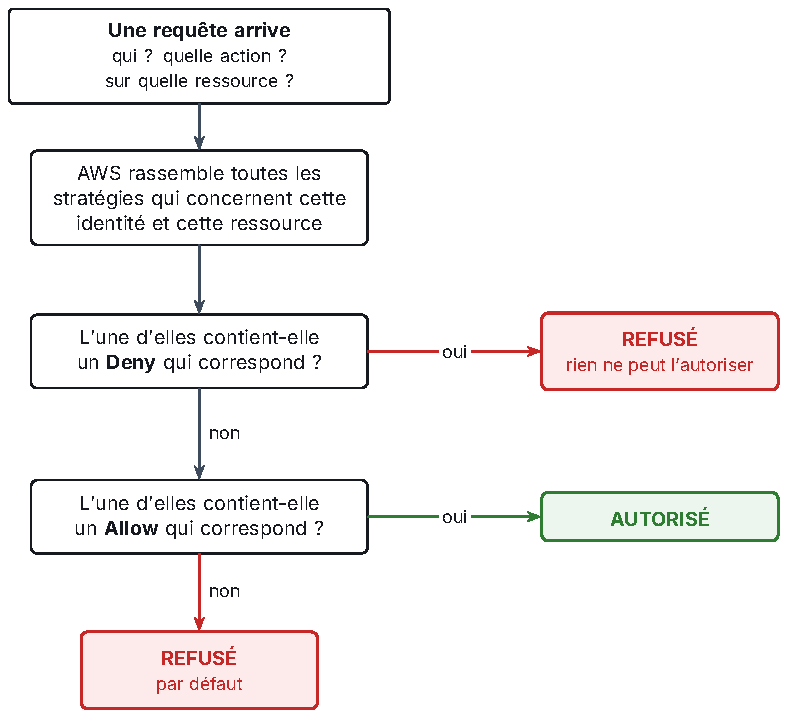
\includegraphics[height=.64\textheight]{evaluation-iam}
    \end{column}
    \begin{column}{.52\textwidth}
      \begin{itemize}
        \setlength{\itemsep}{.6em}
        \item Par défaut : tout est refusé
        \item Un \texttt{Allow} explicite lève le refus
        \item Un \texttt{Deny} explicite l'emporte toujours
        \item Toutes les stratégies applicables sont évaluées ensemble
      \end{itemize}
    \end{column}
  \end{columns}
  \lien{https://docs.aws.amazon.com/IAM/latest/UserGuide/reference_policies_evaluation-logic.html}
\end{frame}

\begin{frame}{ARN : Amazon Resource Name}
  \begin{itemize}
    \item Identifiant unique de toute ressource AWS
    \item Format : \texttt{arn:aws:\emph{service}:\emph{région}:\emph{compte}:\emph{ressource}}
  \end{itemize}
  \medskip
  \renewcommand{\arraystretch}{1.35}
  \begin{tabularx}{\textwidth}{@{}l>{\raggedright\arraybackslash}X@{}}
    \toprule
    \texttt{arn:aws:iam::123456789012:user/camille} & IAM : global, pas de région \\
    \texttt{arn:aws:ec2:eu-west-3:123456789012:instance/i-0abc} & une instance à Paris \\
    \texttt{arn:aws:s3:::galerie-camille} & un bucket : ni région ni compte \\
    \texttt{arn:aws:s3:::galerie-camille/*} & les objets du bucket \\ \bottomrule
  \end{tabularx}
\end{frame}

\begin{frame}{Clés d'accès et identifiants temporaires}
  \centering
  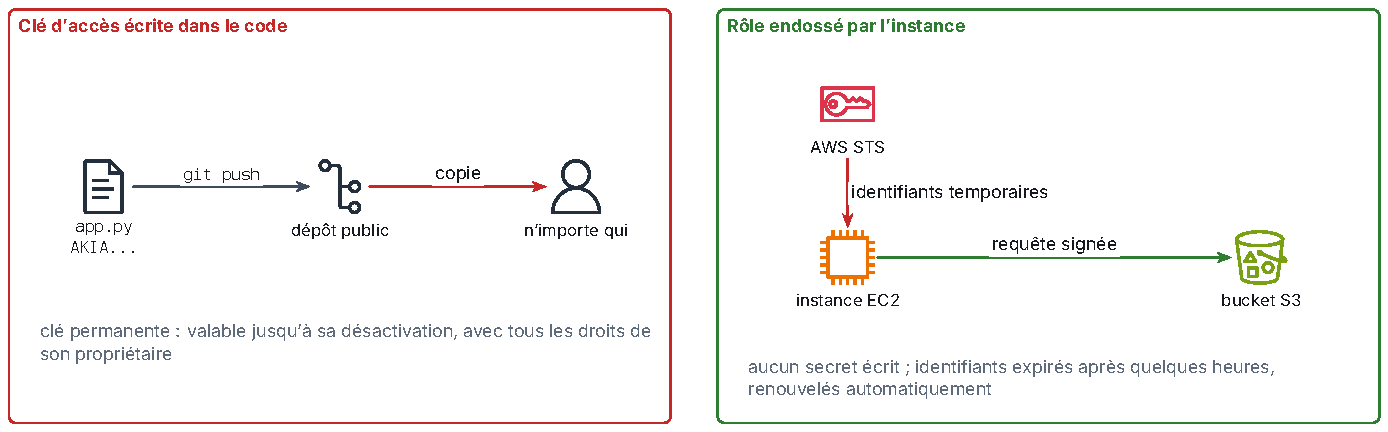
\includegraphics[width=.7\textwidth]{cle-vs-role}\par\medskip
  \raggedright
  \begin{itemize}
    \item Clé permanente (\texttt{AKIA...}) : valable jusqu'à sa désactivation
    \item Identifiant temporaire (\texttt{ASIA...}) : expire après quelques heures
    \item Clé publiée sur GitHub : mise en quarantaine par AWS en une dizaine de secondes
  \end{itemize}
  \source{Unit 42, « From Exposure to Lockdown » ; Meli et al., « How Bad Can It Git? », NDSS 2019.}
\end{frame}

\begin{frame}{Bonnes pratiques IAM}
  \begin{itemize}
    \setlength{\itemsep}{.45em}
    \item Moindre privilège : uniquement les droits nécessaires à la tâche
    \item Droits attribués aux groupes, pas aux utilisateurs
    \item Rôles et identifiants temporaires plutôt que clés d'accès
    \item MFA pour toutes les personnes
    \item Fédération d'identités (IAM Identity Center) pour les personnes en entreprise
    \item Suppression des utilisateurs, clés et droits inutilisés
    \item Comptes séparés par environnement (développement, production)
  \end{itemize}
  \bigskip
  \attention Ne jamais versionner de clé d'accès dans un dépôt Git
  \lien{https://docs.aws.amazon.com/IAM/latest/UserGuide/best-practices.html}
\end{frame}

\begin{frame}{Outils IAM}
  \renewcommand{\arraystretch}{1.45}
  \begin{tabularx}{\textwidth}{@{}>{\raggedright\arraybackslash}p{4.6cm}>{\raggedright\arraybackslash}X@{}}
    \toprule
    \textbf{IAM Policy Simulator} & tester une stratégie sans exécuter d'action \\
    \textbf{IAM Access Analyzer} & détecter les accès publics ou externes, générer des stratégies à partir de l'activité \\
    \textbf{Dernier accès} (\emph{last accessed}) & services utilisés par une identité, droits superflus \\
    \textbf{CloudTrail} & journal des appels d'API : qui, quoi, quand, d'où (90 jours gratuits) \\ \bottomrule
  \end{tabularx}
\end{frame}

% ---- réseau ---------------------------------------------------------------
\begin{frame}{VPC : Virtual Private Cloud}
  \begin{itemize}
    \setlength{\itemsep}{.5em}
    \item Réseau virtuel privé et isolé, propre au compte, dans une région
    \item Plage d'adresses en notation CIDR, par exemple \texttt{10.0.0.0/16}
    \item Contient les sous-réseaux, tables de routage, passerelles
    \item Socle de toutes les ressources réseau : EC2, RDS, ELB...
    \item Plusieurs VPC par compte (5 par région par défaut)
  \end{itemize}
  \bigskip
  \textbf{VPC par défaut} : créé dans chaque région, \texttt{172.31.0.0/16}, un sous-réseau public par AZ, passerelle Internet déjà attachée
\end{frame}

\begin{frame}{Sous-réseaux et accès Internet}
  \begin{itemize}
    \setlength{\itemsep}{.45em}
    \item Sous-réseau : plage d'adresses du VPC, dans \textbf{une seule} AZ (ex. \texttt{10.0.1.0/24})
    \item \textbf{Public} : route vers une passerelle Internet
    \item \textbf{Privé} : pas d'accès entrant depuis Internet
    \item \textbf{Internet Gateway} : relie le VPC à Internet, gratuite
    \item \textbf{NAT Gateway} : sortie vers Internet pour les sous-réseaux privés ; environ 0,045 \$/h + 0,045 \$/Go traité (\texttt{us-east-1})
    \item Adresse IPv4 publique : facturée 0,005 \$/h
  \end{itemize}
  \source{AWS, \emph{Amazon VPC pricing}.}
\end{frame}

\begin{frame}{Topologie réseau type}
  \centering
  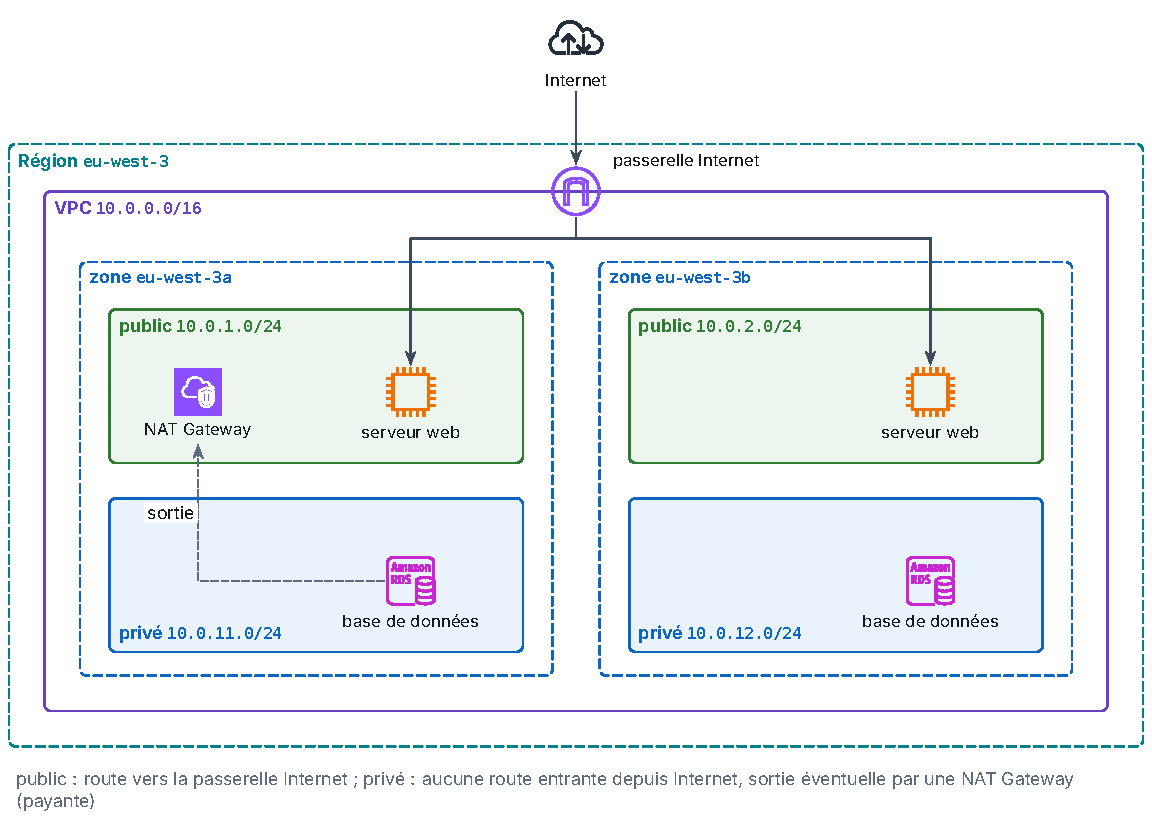
\includegraphics[height=.8\textheight]{vpc-topologie}
\end{frame}

\begin{frame}{Notation CIDR}
  \renewcommand{\arraystretch}{1.4}
  \begin{tabular}{@{}l l r@{}}
    \toprule
    \textbf{Notation} & \textbf{Signification} & \textbf{Adresses} \\ \midrule
    \texttt{10.0.0.0/16} & bloc d'un VPC & 65 536 \\
    \texttt{10.0.1.0/24} & bloc d'un sous-réseau & 256 (251 utilisables sur AWS) \\
    \texttt{203.0.113.25/32} & une seule adresse & 1 \\
    \texttt{0.0.0.0/0} & toutes les adresses IPv4 & \\
    \texttt{::/0} & toutes les adresses IPv6 & \\ \bottomrule
  \end{tabular}
  \bigskip
  \begin{itemize}
    \item AWS réserve 5 adresses par sous-réseau
  \end{itemize}
\end{frame}

\begin{frame}{Security Groups}
  \begin{itemize}
    \setlength{\itemsep}{.45em}
    \item Pare-feu virtuel attaché à l'interface réseau d'une ressource (instance, base RDS...)
    \item Règles : protocole, port, source (CIDR ou autre Security Group)
    \item Uniquement des autorisations
    \item Par défaut : entrant interdit, sortant autorisé
    \item \textbf{Avec état} (\emph{stateful}) : la réponse à une connexion autorisée est autorisée
    \item Modifications appliquées immédiatement
    \item Plusieurs Security Groups par ressource : règles cumulées
  \end{itemize}
  \lien{https://docs.aws.amazon.com/vpc/latest/userguide/vpc-security-groups.html}
\end{frame}

\begin{frame}{Security Group d'un serveur web}
  \centering
  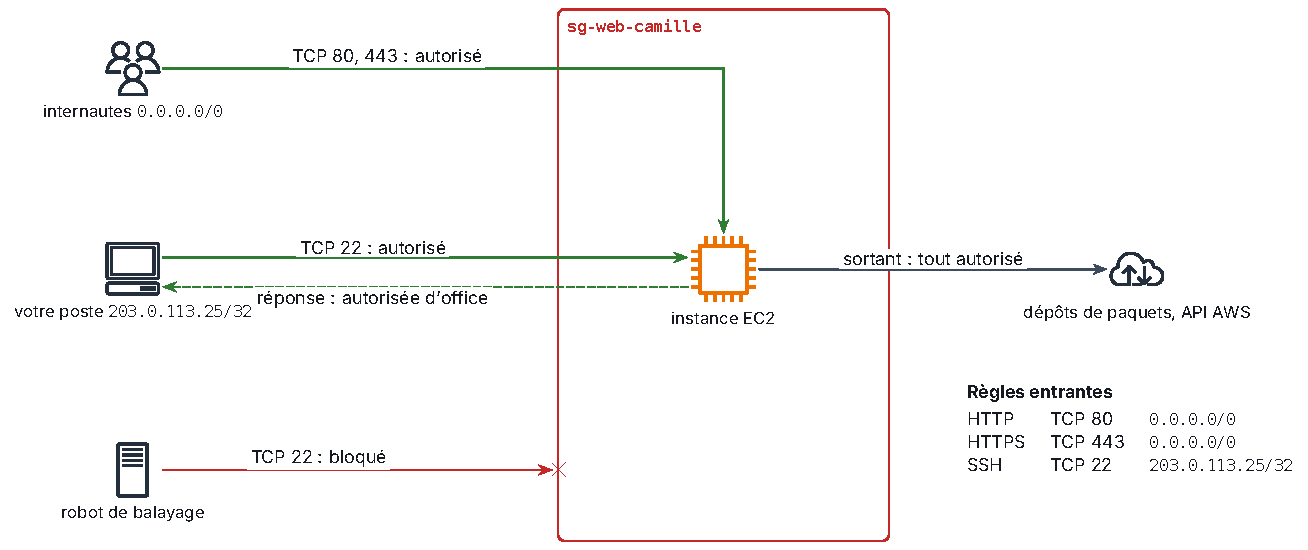
\includegraphics[width=.95\textwidth]{security-group}
\end{frame}

\begin{frame}{Security Groups et NACL}
  \renewcommand{\arraystretch}{1.4}
  \begin{tabularx}{\textwidth}{@{}>{\raggedright\arraybackslash}p{3.4cm}>{\raggedright\arraybackslash}X>{\raggedright\arraybackslash}X@{}}
    \toprule
    & \textbf{Security Group} & \textbf{Network ACL} \\ \midrule
    Portée & interface réseau (instance) & sous-réseau \\
    Règles & autorisations seulement & autorisations et interdictions \\
    État & avec état & sans état : trafic retour à autoriser \\
    Évaluation & toutes les règles & par numéro de règle, la première qui correspond \\
    Par défaut & entrant refusé, sortant autorisé & NACL par défaut : tout autorisé \\ \bottomrule
  \end{tabularx}
\end{frame}

\begin{frame}{Bonnes pratiques réseau}
  \begin{itemize}
    \setlength{\itemsep}{.5em}
    \item N'ouvrir que les ports nécessaires
    \item SSH (22) limité à une adresse précise, jamais \texttt{0.0.0.0/0}
    \item Bases de données dans des sous-réseaux privés
    \item Source = Security Group plutôt que plage d'adresses entre niveaux d'une application
    \item Session Manager (Systems Manager) : administration sans port SSH ouvert
  \end{itemize}
  \bigskip
  \attention L'espace IPv4 complet peut être balayé en moins de 45 minutes depuis une seule machine (ZMap)
  \source{Durumeric et al., « ZMap: Fast Internet-Wide Scanning and its Security Applications », USENIX Security 2013.}
\end{frame}

\diapotp{2}{Utilisateurs, droits et pare-feu}{%
  \item Stratégie sur mesure, groupe et utilisateur au moindre privilège
  \item Tests dans la console et dans CloudShell
  \item Simulateur de stratégies, refus explicite
  \item Security Group du serveur web}


% =====================================================================
%  Module 3 : Calcul, Amazon EC2
% =====================================================================
\section{Calcul : Amazon EC2}

\begin{frame}{Amazon EC2 : Elastic Compute Cloud}
  \begin{itemize}
    \setlength{\itemsep}{.55em}
    \item Machines virtuelles (\emph{instances}) à la demande : service IaaS, lancé en 2006
    \item Démarrage en quelques dizaines de secondes à partir d'une image (AMI)
    \item Plus de 1 200 types d'instances : usage général, calcul, mémoire, stockage, GPU
    \item Linux, Windows, macOS ; processeurs Intel, AMD, AWS Graviton (Arm)
    \item Facturation à la seconde pour Linux (minimum 60 s)
  \end{itemize}
  \lien{https://docs.aws.amazon.com/AWSEC2/latest/UserGuide/concepts.html}
\end{frame}

\begin{frame}{Caractéristiques d'une instance}
  \renewcommand{\arraystretch}{1.45}
  \begin{tabularx}{\textwidth}{@{}>{\raggedright\arraybackslash}p{3.4cm}>{\raggedright\arraybackslash}X@{}}
    \toprule
    \textbf{Calcul} & nombre de vCPU, génération et fabricant du processeur \\
    \textbf{Mémoire} & de 0,5 Gio (\texttt{t3.nano}) à plusieurs Tio \\
    \textbf{Stockage} & volumes EBS (réseau) et, selon le type, disques locaux (\emph{instance store}) \\
    \textbf{Réseau} & bande passante, de quelques Gbit/s à plusieurs centaines \\
    \textbf{Placement} & une région, une AZ, un sous-réseau \\ \bottomrule
  \end{tabularx}
\end{frame}

\begin{frame}{Nomenclature des types d'instances}
  \centering
  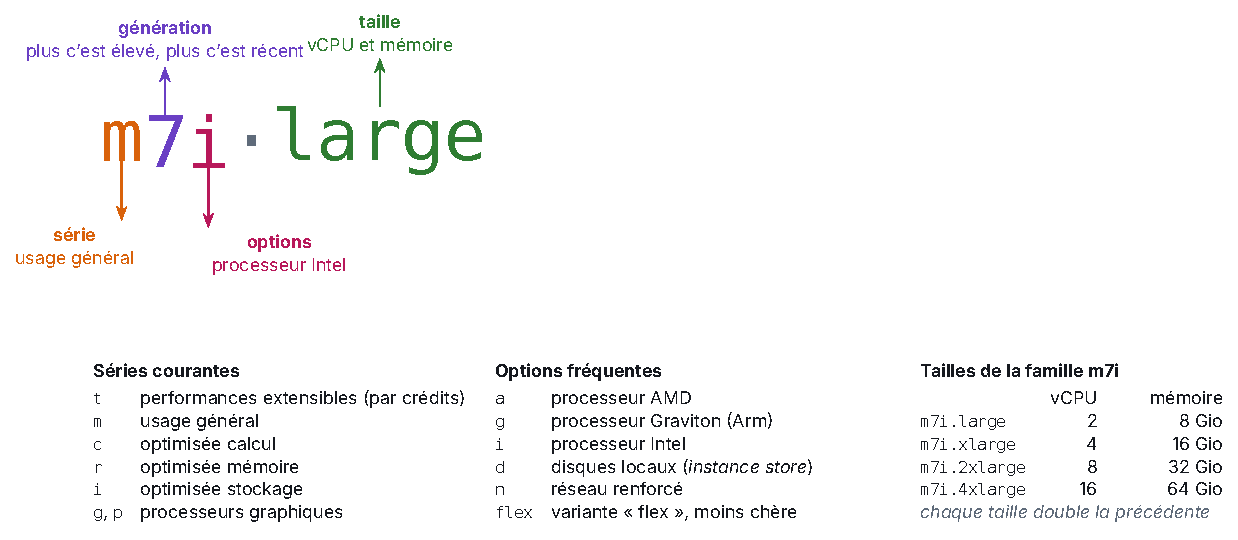
\includegraphics[width=.96\textwidth]{type-instance}
  \lien{https://docs.aws.amazon.com/ec2/latest/instancetypes/instance-type-names.html}
\end{frame}

\begin{frame}{Familles d'instances}
  \renewcommand{\arraystretch}{1.12}
  \begin{tabularx}{\textwidth}{@{}>{\raggedright\arraybackslash}p{2.8cm}>{\raggedright\arraybackslash}p{4.4cm}>{\raggedright\arraybackslash}X@{}}
    \toprule
    \textbf{Exemples} & \textbf{Famille} & \textbf{Usages} \\ \midrule
    \texttt{t3}, \texttt{t4g} & extensible (crédits CPU) & petits sites, tests \\
    \texttt{m7i}, \texttt{m8g} & usage général & serveurs d'applications \\
    \texttt{c7i}, \texttt{c8g} & optimisée calcul & calcul intensif, encodage \\
    \texttt{r7i}, \texttt{r8g} & optimisée mémoire & bases de données, caches \\
    \texttt{i4i}, \texttt{d3} & optimisée stockage & bases NoSQL, entrepôts \\
    \texttt{g6}, \texttt{p5} & accélérée (GPU) & apprentissage automatique \\
    \texttt{inf2}, \texttt{trn2} & puces Inferentia, Trainium & inférence, entraînement \\ \bottomrule
  \end{tabularx}
  \smallskip
  \attention Changer de type demande d'arrêter puis redémarrer l'instance
\end{frame}

\begin{frame}{Instances à performances extensibles (T)}
  \begin{columns}[c]
    \begin{column}{.58\textwidth}
      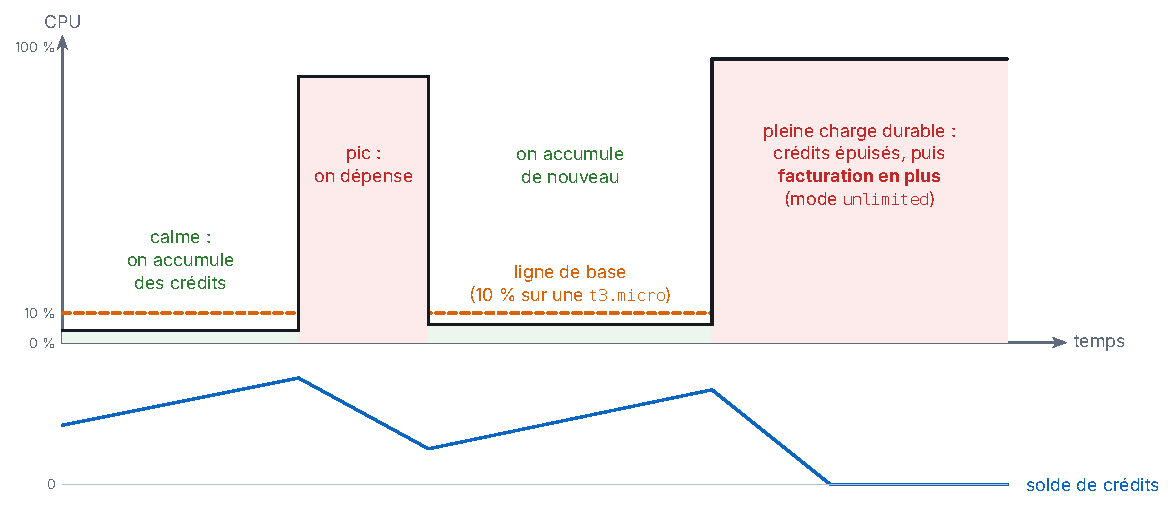
\includegraphics[width=\textwidth]{credits-cpu}
    \end{column}
    \begin{column}{.4\textwidth}
      \begin{itemize}
        \setlength{\itemsep}{.5em}
        \item Ligne de base : 10 \% par vCPU pour une \texttt{t3.micro}
        \item Crédits accumulés sous la ligne de base (12 par heure), dépensés au-dessus
        \item Mode \texttt{standard} : bridage une fois les crédits épuisés
        \item Mode \texttt{unlimited} (défaut des \texttt{t3}) : surplus facturé
      \end{itemize}
    \end{column}
  \end{columns}
  \lien{https://docs.aws.amazon.com/AWSEC2/latest/UserGuide/burstable-performance-instances.html}
\end{frame}

\begin{frame}{Modes d'achat}
  \renewcommand{\arraystretch}{1.4}
  \begin{tabularx}{\textwidth}{@{}>{\raggedright\arraybackslash}p{3.6cm}>{\raggedright\arraybackslash}X >{\raggedright\arraybackslash}p{2.6cm}@{}}
    \toprule
    \textbf{Mode} & \textbf{Principe} & \textbf{Remise} \\ \midrule
    On-Demand & à la seconde, sans engagement & aucune \\
    Savings Plans & engagement de dépense horaire sur 1 ou 3 ans & jusqu'à 72 \% \\
    Instances réservées & engagement sur un type d'instance, 1 ou 3 ans & jusqu'à 72 \% \\
    Spot & capacité inutilisée, reprise avec préavis de 2 minutes & jusqu'à 90 \% \\
    Hôtes dédiés & serveur physique réservé (licences, conformité) & \\ \bottomrule
  \end{tabularx}
  \lien{https://aws.amazon.com/ec2/pricing/}
\end{frame}

\begin{frame}{AMI : Amazon Machine Image}
  \begin{itemize}
    \setlength{\itemsep}{.45em}
    \item Modèle de démarrage : système d'exploitation, configuration, logiciels
    \item Propre à une région (identifiant \texttt{ami-...}) et à une architecture (x86\_64 ou arm64)
    \item Sources : AWS, AWS Marketplace, communauté, AMI personnalisées
    \item AMI personnalisée : EC2 Image Builder, Packer, ou instantané d'une instance
    \item Amazon Linux 2023 : distribution d'AWS, \texttt{dnf}, utilisateur \texttt{ec2-user}, CLI \texttt{aws} incluse
  \end{itemize}
  \bigskip
  \attention Amazon Linux 2 n'est plus maintenu depuis le 30/06/2026
  \par\attention Une AMI de la Marketplace est une dépendance externe : vérifier son éditeur
  \source{AWS, \emph{Amazon Linux 2 FAQs}.}
\end{frame}

\begin{frame}{AMI, instances et volumes}
  \centering
  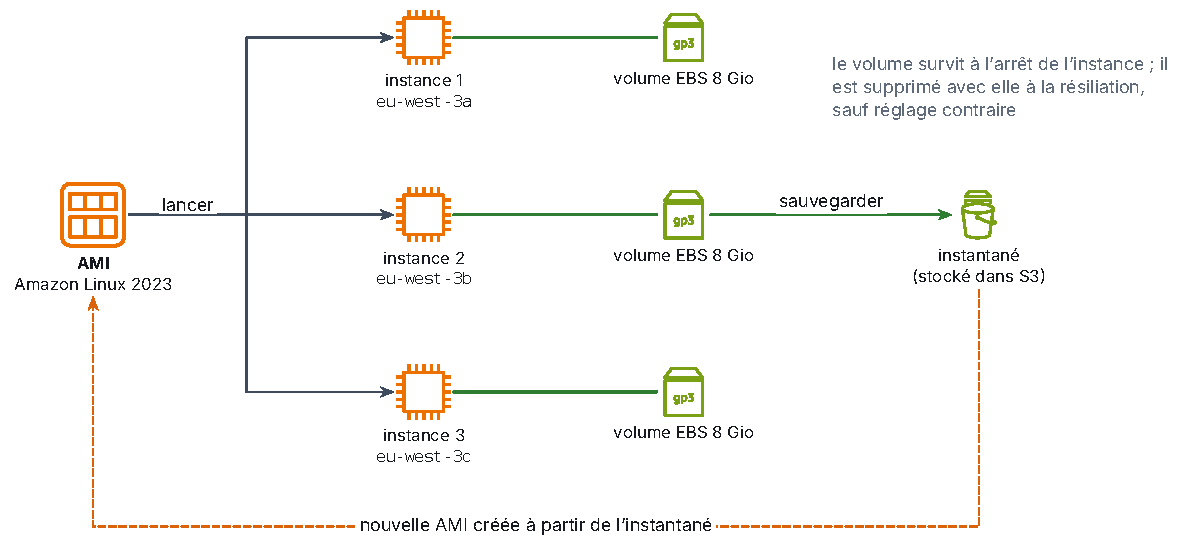
\includegraphics[width=.95\textwidth]{ami-instance-ebs}
\end{frame}

\begin{frame}{Stockage d'une instance}
  \renewcommand{\arraystretch}{1.45}
  \begin{tabularx}{\textwidth}{@{}>{\raggedright\arraybackslash}p{3.4cm}>{\raggedright\arraybackslash}X>{\raggedright\arraybackslash}X@{}}
    \toprule
    & \textbf{Volume EBS} & \textbf{Instance store} \\ \midrule
    Nature & disque réseau & disque physique du serveur hôte \\
    Persistance & survit à l'arrêt de l'instance & perdu à l'arrêt ou à la résiliation \\
    Instantané & oui (stocké dans S3) & non \\
    Usage & disque racine, données & cache, fichiers temporaires \\ \bottomrule
  \end{tabularx}
  \bigskip
  \begin{itemize}
    \item Volume racine supprimé à la résiliation par défaut (\emph{DeleteOnTermination})
  \end{itemize}
\end{frame}

\begin{frame}{Paires de clés et connexion}
  \begin{columns}[c]
    \begin{column}{.56\textwidth}
      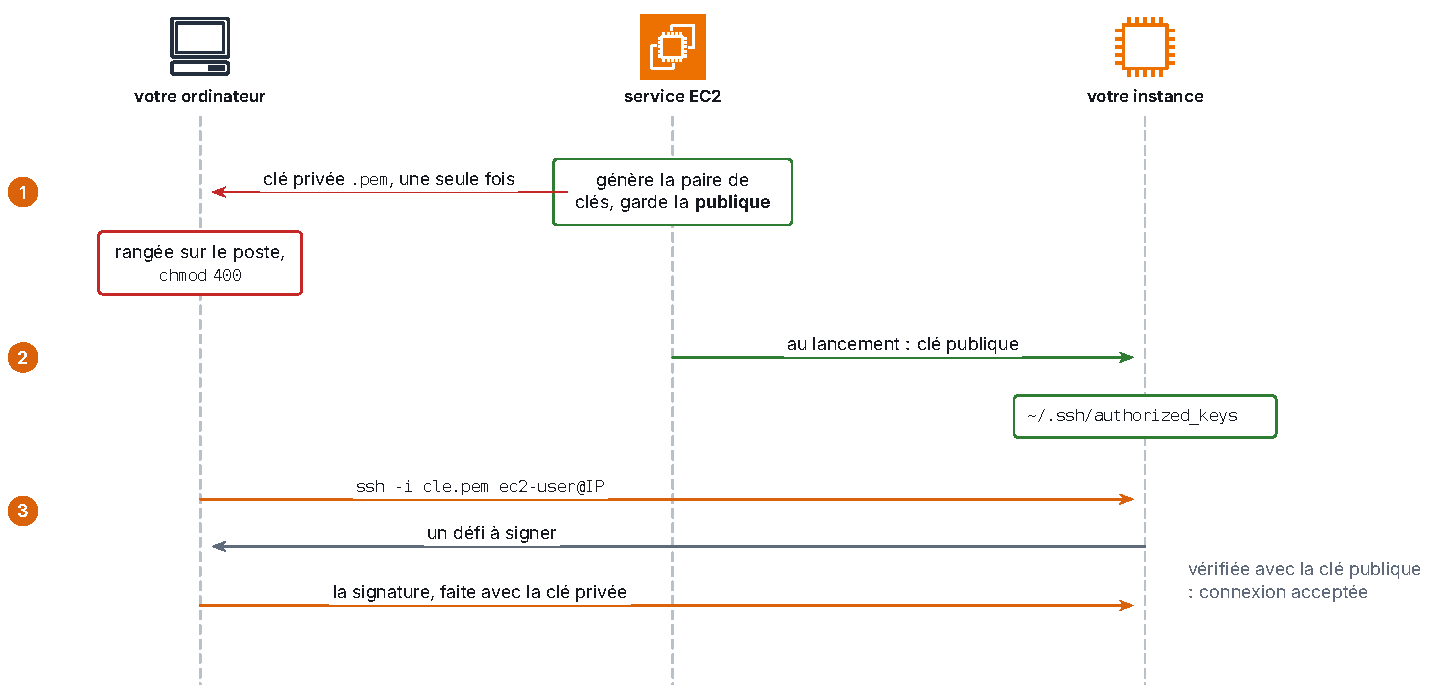
\includegraphics[width=\textwidth]{ssh-cles}
    \end{column}
    \begin{column}{.42\textwidth}
      \begin{itemize}
        \setlength{\itemsep}{.45em}
        \item Types : RSA ou ED25519
        \item Clé privée remise une seule fois, non conservée par AWS
        \item Clé publique copiée dans \texttt{authorized\_keys} au démarrage
        \item Permissions du fichier : \texttt{chmod 400}
      \end{itemize}
    \end{column}
  \end{columns}
\end{frame}

\begin{frame}{Se connecter à une instance Linux}
  \renewcommand{\arraystretch}{1.45}
  \begin{tabularx}{\textwidth}{@{}>{\raggedright\arraybackslash}p{3.8cm}>{\raggedright\arraybackslash}X>{\raggedright\arraybackslash}X@{}}
    \toprule
    \textbf{Méthode} & \textbf{Prérequis} & \textbf{Remarque} \\ \midrule
    SSH & clé privée, port 22 ouvert à votre adresse & méthode de référence \\
    EC2 Instance Connect & port 22 ouvert aux adresses d'AWS & clé temporaire poussée par l'API \\
    Session Manager & rôle avec \texttt{AmazonSSMManagedInstanceCore} & aucun port entrant \\
    EC2 Serial Console & droits IAM dédiés & dépannage (démarrage, réseau) \\ \bottomrule
  \end{tabularx}
\end{frame}

\begin{frame}{Cycle de vie d'une instance}
  \centering
  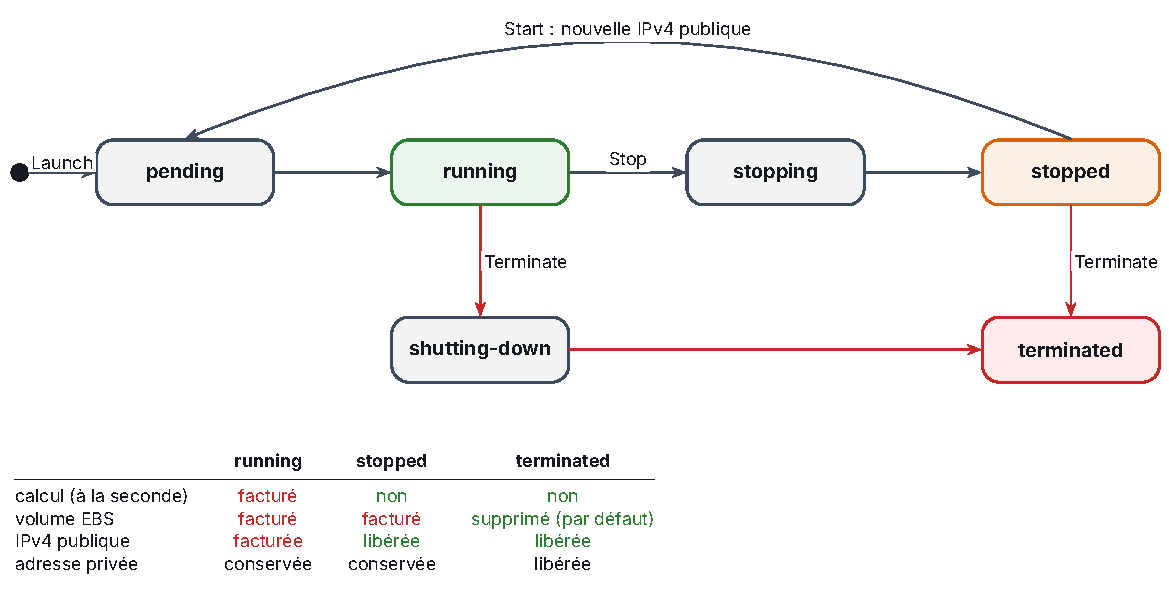
\includegraphics[height=.78\textheight]{cycle-vie}
\end{frame}

\begin{frame}{Adresses IP}
  \begin{itemize}
    \setlength{\itemsep}{.5em}
    \item \textbf{Adresse privée} : dans le sous-réseau, conservée jusqu'à la résiliation
    \item \textbf{IPv4 publique} : attribuée au démarrage, \textbf{change} après un arrêt puis un démarrage
    \item \textbf{Elastic IP} : adresse publique fixe, réservée dans le compte
    \item \textbf{IPv6} : adresses publiques, non facturées
    \item Toute IPv4 publique est facturée, Elastic IP non attachée comprise
  \end{itemize}
  \bigskip
  \attention L'instance ne voit que son adresse privée : la passerelle Internet traduit l'adresse publique
\end{frame}

\begin{frame}[fragile]{User data}
  \begin{itemize}
    \item Script exécuté par \texttt{cloud-init}, en \texttt{root}, au premier démarrage
    \item Installation et configuration automatiques
    \item Journal : \texttt{/var/log/cloud-init-output.log}
  \end{itemize}
  \begin{terminal}
\#!/bin/bash\\
dnf install -y nginx\\
systemctl enable --now nginx
  \end{terminal}
  \begin{itemize}
    \item Instance reproductible : on la remplace au lieu de la réparer
  \end{itemize}
  \attention Ne pas mettre de secret dans le user data : il est lisible via le service de métadonnées
\end{frame}

\begin{frame}{Service de métadonnées (IMDS)}
  \centering
  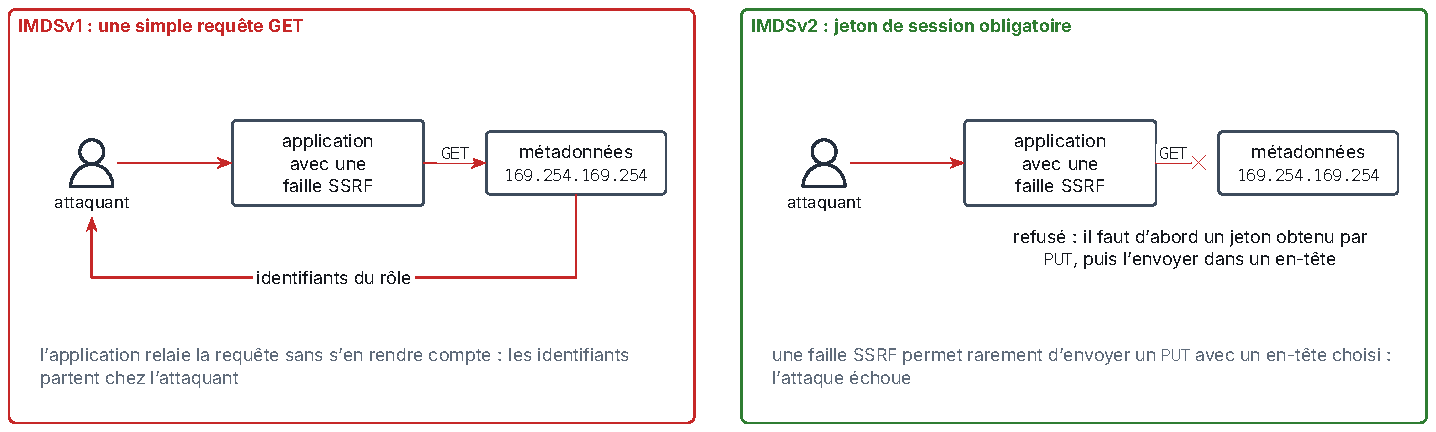
\includegraphics[width=.84\textwidth]{imds}\par\medskip
  \raggedright
  \begin{itemize}
    \item \texttt{169.254.169.254} : identifiant, type, AZ, adresses, identifiants du rôle
    \item IMDSv2 (2019) : jeton obtenu par \texttt{PUT}, puis en-tête obligatoire ; exigé par défaut sur Amazon Linux 2023
  \end{itemize}
  \source{C. MacCárthaigh, « Add defense in depth against open firewalls, reverse proxies, and SSRF vulnerabilities », AWS Security Blog, 2019.}
\end{frame}

\begin{frame}{Tags}
  \begin{itemize}
    \setlength{\itemsep}{.5em}
    \item Paires clé-valeur sur presque toutes les ressources (\texttt{Name}, \texttt{Proprietaire}, \texttt{Projet}...)
    \item Usages :
    \begin{itemize}
      \item retrouver et grouper des ressources
      \item répartition des coûts par projet ou par équipe
      \item contrôle d'accès par attributs (ABAC) : conditions \texttt{aws:ResourceTag}
    \end{itemize}
    \item Convention de nommage à définir dès le départ
  \end{itemize}
  \bigskip
  \attention Pas de données sensibles dans les tags
\end{frame}

\begin{frame}{Supervision}
  \begin{itemize}
    \setlength{\itemsep}{.5em}
    \item \textbf{Status checks} : contrôles système (hôte) et instance (système d'exploitation)
    \item \textbf{CloudWatch} : métriques CPU, réseau, disque toutes les 5 minutes (1 minute en option)
    \item Mémoire et espace disque : agent CloudWatch à installer
    \item Alarmes : notification ou action (arrêt, redémarrage, mise à l'échelle)
  \end{itemize}
\end{frame}

\begin{frame}{Exemple de coût : \texttt{t3.micro} à Paris}
  \begin{center}
  \renewcommand{\arraystretch}{1.3}
  \begin{tabular}{@{}lrr@{}}
    \toprule
    & \textbf{Une semaine} & \textbf{Un mois} \\ \midrule
    Instance (\(\approx\) 0,012 \$/h) & 2,02 \$ & 8,76 \$ \\
    IPv4 publique (0,005 \$/h) & 0,84 \$ & 3,65 \$ \\
    EBS gp3 8 Go (\(\approx\) 0,09 \$/Go-mois) & 0,17 \$ & 0,72 \$ \\ \midrule
    \textbf{Total} & \textbf{\(\approx\) 3 \$} & \textbf{\(\approx\) 13 \$} \\ \bottomrule
  \end{tabular}
  \end{center}
  \source{ordres de grandeur des tarifs à la demande ; valeurs exactes sur \url{https://aws.amazon.com/ec2/pricing/on-demand/}}
\end{frame}

\diapotp{3}{Un serveur web sur EC2}{%
  \item Paire de clés, lancement d'une instance Amazon Linux 2023
  \item Connexion SSH, installation de Nginx
  \item Lecture des métadonnées (IMDSv2)
  \item Arrêt, redémarrage, relance par user data}


% =====================================================================
%  Module 4 : Stockage, bases de données et messages
% =====================================================================
\section{Stockage, bases de données et messages}

\begin{frame}{Trois types de stockage}
  \centering
  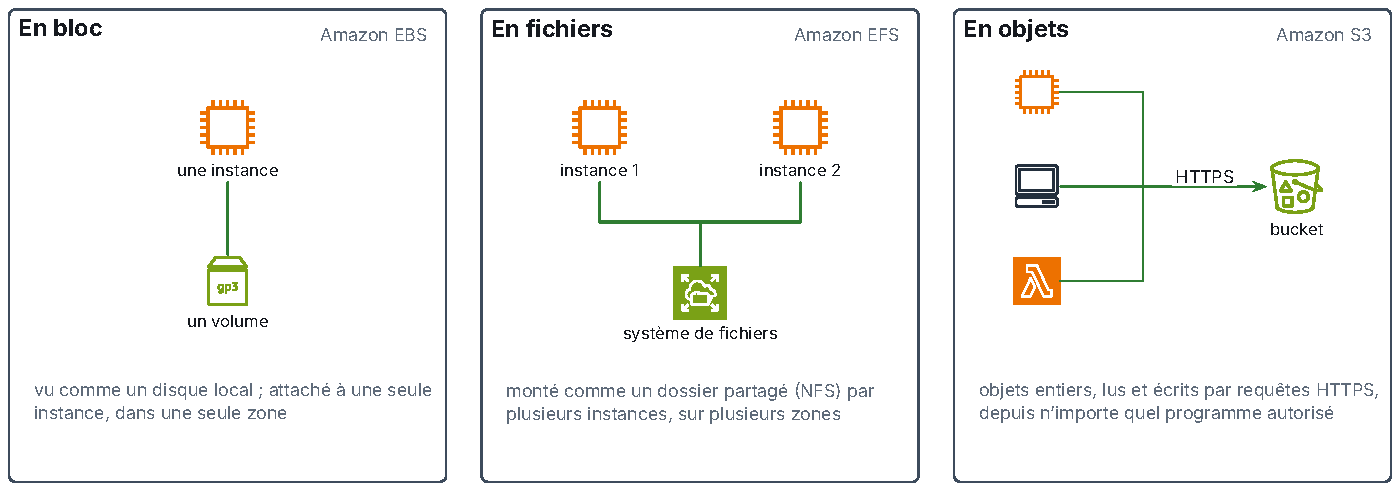
\includegraphics[width=.96\textwidth]{stockage-types}
\end{frame}

\begin{frame}{Amazon S3 : Simple Storage Service}
  \begin{itemize}
    \setlength{\itemsep}{.45em}
    \item Stockage objet, accessible par API HTTPS
    \item \textbf{Objet} : clé + données + métadonnées ; de 0 octet à 50 To
    \item Envoi en une requête jusqu'à 5 Go, au-delà téléversement en plusieurs parties
    \item \textbf{Bucket} : conteneur d'objets, créé dans une région
    \item Nom de bucket unique au monde (3 à 63 caractères, minuscules)
    \item Cohérence forte en lecture après écriture depuis 2020
    \item Plus de 500 000 milliards d'objets stockés, plus de 200 millions de requêtes par seconde
  \end{itemize}
  \source{AWS, \emph{Amazon S3 FAQs} ; S. Stormacq, « Twenty years of Amazon S3 », AWS News Blog, 2026.}
\end{frame}

\begin{frame}{Buckets, clés et préfixes}
  \centering
  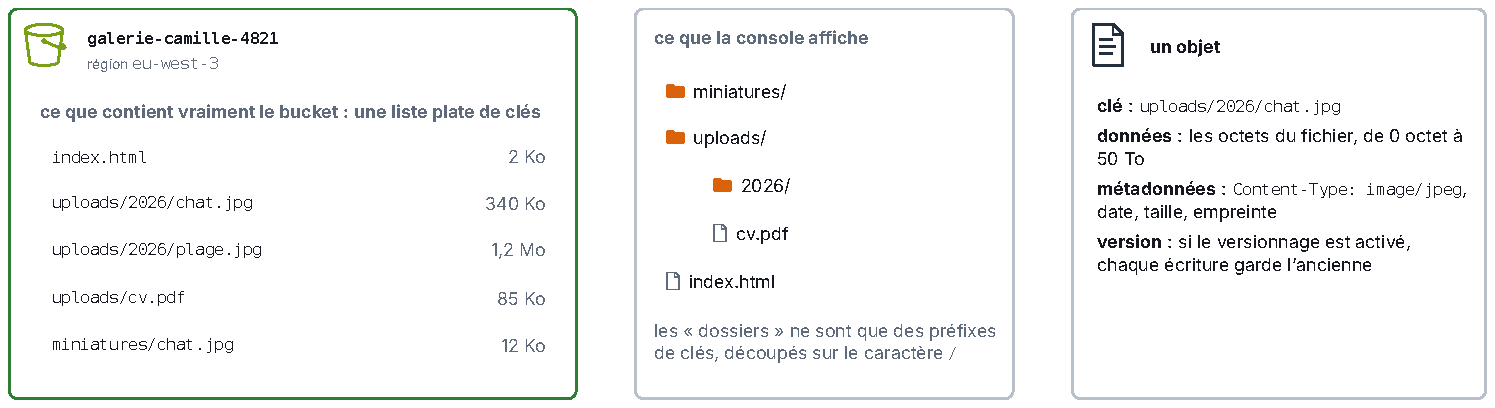
\includegraphics[width=.96\textwidth]{s3-modele}\par\medskip
  \raggedright
  \begin{itemize}
    \item Pas de dossiers : des clés à plat, regroupées par préfixe dans la console
  \end{itemize}
\end{frame}

\begin{frame}{Classes de stockage S3}
  \renewcommand{\arraystretch}{1.12}
  \begin{tabularx}{\textwidth}{@{}>{\raggedright\arraybackslash}p{5.4cm}>{\raggedright\arraybackslash}X@{}}
    \toprule
    \textbf{Classe} & \textbf{Usage} \\ \midrule
    S3 Standard & données lues fréquemment (classe par défaut) \\
    S3 Intelligent-Tiering & accès imprévisible, niveaux automatiques \\
    S3 Standard-IA & lectures rares, accès immédiat \\
    S3 One Zone-IA & comme Standard-IA, dans une seule AZ \\
    S3 Glacier Instant Retrieval & archives lues environ une fois par trimestre \\
    S3 Glacier Flexible Retrieval & archives, récupération en minutes à heures \\
    S3 Glacier Deep Archive & archives longues, récupération en 12 à 48 h \\
    S3 Express One Zone & latence très faible, une seule AZ \\ \bottomrule
  \end{tabularx}
  \source{\url{https://aws.amazon.com/s3/storage-classes/}}
\end{frame}

\begin{frame}{Durabilité et disponibilité}
  \begin{itemize}
    \setlength{\itemsep}{.55em}
    \item Durabilité conçue pour 99,999999999 \% par an (11 neuf)
    \item Soit une probabilité de perte de \(10^{-11}\) par objet et par an
    \item Avec 10 millions d'objets : une perte attendue tous les 10 000 ans environ
    \item Données copiées sur plusieurs AZ (sauf classes One Zone)
    \item SLA de disponibilité de S3 Standard : 99,9 \%
  \end{itemize}
  \bigskip
  \attention La durabilité protège contre les pannes matérielles, pas contre une suppression : activer le versionnage
\end{frame}

\begin{frame}{Fonctionnalités de S3}
  \begin{itemize}
    \setlength{\itemsep}{.45em}
    \item \textbf{Versionnage} : conservation des versions précédentes de chaque objet
    \item \textbf{Cycle de vie} : changement de classe ou suppression automatique selon l'âge
    \item \textbf{Réplication} : vers un autre bucket, dans la même région ou une autre
    \item \textbf{Chiffrement} : SSE-S3 appliqué par défaut depuis janvier 2023, SSE-KMS en option
    \item \textbf{Notifications d'événements} : vers SQS, SNS, Lambda, EventBridge
    \item \textbf{Hébergement de site statique}
    \item \textbf{Object Lock} : écriture unique, lecture multiple (WORM)
  \end{itemize}
\end{frame}

\begin{frame}{Contrôle d'accès à S3}
  \begin{itemize}
    \setlength{\itemsep}{.45em}
    \item Stratégies IAM de l'appelant (utilisateur, rôle)
    \item Stratégie de bucket (basée sur la ressource)
    \item \textbf{Block Public Access} : activé par défaut sur les nouveaux buckets depuis avril 2023
    \item ACL désactivées par défaut (\emph{Object Ownership : bucket owner enforced})
    \item URL présignée : accès temporaire à un objet précis
  \end{itemize}
  \bigskip
  \attention Juin 2017 : bucket public d'un sous-traitant de Verizon, données de 6 à 14 millions de clients exposées
  \source{AWS, « Amazon S3 now applies two security best practices to all new buckets by default », 2023 ; UpGuard, « Cloud Leak: How A Verizon Partner Exposed Millions of Customer Accounts », 2017.}
\end{frame}

\begin{frame}{Qui peut lire un objet ?}
  \centering
  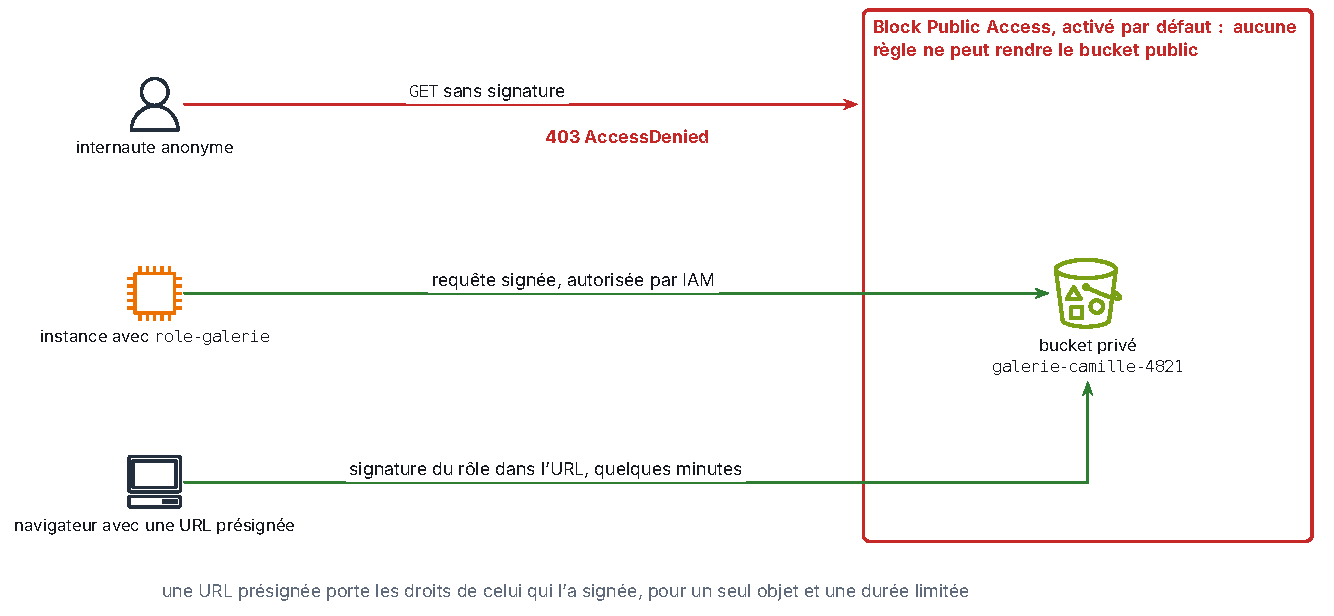
\includegraphics[width=.95\textwidth]{s3-acces}
\end{frame}

\begin{frame}[fragile]{Stratégie de bucket}
  Exemple : refuser toute requête qui n'utilise pas HTTPS
\begin{lstlisting}[language=json]
{
  "Version": "2012-10-17",
  "Statement": [{
    "Sid": "HTTPSUniquement",
    "Effect": "Deny",
    "Principal": "*",
    "Action": "s3:*",
    "Resource": ["arn:aws:s3:::galerie-camille",
                 "arn:aws:s3:::galerie-camille/*"],
    "Condition": { "Bool": { "aws:SecureTransport": "false" } }
  }]
}
\end{lstlisting}
  \lien{https://docs.aws.amazon.com/AmazonS3/latest/userguide/example-bucket-policies.html}
\end{frame}

\begin{frame}{Tarification de S3}
  \begin{itemize}
    \setlength{\itemsep}{.5em}
    \item Volume stocké par mois, selon la classe : un peu plus de 0,02 \$/Go-mois en Standard
    \item Requêtes : \texttt{PUT}, \texttt{COPY}, \texttt{LIST} plus chères que \texttt{GET}
    \item Transfert sortant vers Internet ; transfert entrant gratuit
    \item Frais de récupération pour les classes IA et Glacier
    \item Fonctionnalités optionnelles : réplication, analyse, Transfer Acceleration
  \end{itemize}
  \lien{https://aws.amazon.com/s3/pricing/}
\end{frame}

\begin{frame}{Amazon EBS : Elastic Block Store}
  \begin{itemize}
    \setlength{\itemsep}{.45em}
    \item Volume de stockage en bloc, vu comme un disque par l'instance
    \item Dans une seule AZ, répliqué à l'intérieur de cette AZ
    \item Attaché à une instance à la fois (sauf Multi-Attach pour \texttt{io1}/\texttt{io2})
    \item Système de fichiers à créer par l'utilisateur
    \item Instantanés incrémentaux stockés dans S3, copiables entre régions
    \item Chiffrement des volumes et des instantanés (KMS)
  \end{itemize}
  \bigskip
  \attention Pas de multi-AZ : un instantané permet de recréer le volume dans une autre AZ
\end{frame}

\begin{frame}{Types de volumes EBS}
  \renewcommand{\arraystretch}{1.12}
  \begin{tabularx}{\textwidth}{@{}>{\raggedright\arraybackslash}p{3.6cm}>{\raggedright\arraybackslash}p{1.6cm}>{\raggedright\arraybackslash}X >{\raggedright\arraybackslash}p{2.6cm}@{}}
    \toprule
    \textbf{Type} & \textbf{Support} & \textbf{Usage} & \textbf{Taille max.} \\ \midrule
    \texttt{gp3} & SSD & usage général, 3 000 à 80 000 IOPS & 64 Tio \\
    \texttt{gp2} & SSD & génération précédente & 16 Tio \\
    \texttt{io2} Block Express & SSD & bases critiques, jusqu'à 256 000 IOPS & 64 Tio \\
    \texttt{st1} & HDD & débit séquentiel (journaux) & 16 Tio \\
    \texttt{sc1} & HDD & données froides, coût minimal & 16 Tio \\ \bottomrule
  \end{tabularx}
  \source{AWS, \emph{Amazon EBS volume types} ; « Amazon EBS increases the maximum size and provisioned performance of gp3 volumes », 2025.}
\end{frame}

\begin{frame}{Amazon EFS et comparaison}
  \begin{itemize}
    \item EFS : système de fichiers NFS managé, élastique, partagé par plusieurs instances, sur plusieurs AZ
  \end{itemize}
  \medskip
  \renewcommand{\arraystretch}{1.12}
  \begin{tabularx}{\textwidth}{@{}>{\raggedright\arraybackslash}p{2.6cm}>{\raggedright\arraybackslash}X>{\raggedright\arraybackslash}X>{\raggedright\arraybackslash}X@{}}
    \toprule
    & \textbf{S3} & \textbf{EBS} & \textbf{EFS} \\ \midrule
    Type & objet & bloc & fichiers (NFS) \\
    Accès & API HTTPS & une instance & plusieurs instances \\
    Redondance & plusieurs AZ (selon classe) & une AZ & plusieurs AZ \\
    Facturation & volume réel + requêtes & volume provisionné & volume réel \\
    Usage type & fichiers, sauvegardes & disque système, base & dossier partagé \\ \bottomrule
  \end{tabularx}
\end{frame}

% ---- bases de données ------------------------------------------------------
\begin{frame}{Bases relationnelles et NoSQL}
  \renewcommand{\arraystretch}{1.35}
  \begin{tabularx}{\textwidth}{@{}>{\raggedright\arraybackslash}p{2.8cm}>{\raggedright\arraybackslash}X>{\raggedright\arraybackslash}X@{}}
    \toprule
    & \textbf{Relationnel (SQL)} & \textbf{NoSQL} \\ \midrule
    Modèle & tables, schéma fixe, jointures & clé-valeur, document, graphe ; schéma souple \\
    Requêtes & SQL & API propre à chaque moteur \\
    Mise à l'échelle & surtout verticale & horizontale (partitionnement) \\
    Garanties & transactions ACID & souvent cohérence à terme, transactions limitées \\
    Exemples & PostgreSQL, MySQL, Oracle & DynamoDB, MongoDB, Redis, Neo4j \\ \bottomrule
  \end{tabularx}
\end{frame}

\begin{frame}{Bases de données managées sur AWS}
  \renewcommand{\arraystretch}{1.35}
  \begin{tabularx}{\textwidth}{@{}>{\raggedright\arraybackslash}p{4cm}>{\raggedright\arraybackslash}X@{}}
    \toprule
    \textbf{Amazon RDS} & PostgreSQL, MySQL, MariaDB, Oracle, SQL Server, Db2 \\
    \textbf{Amazon Aurora} & compatible PostgreSQL et MySQL, stockage réparti sur 3 AZ \\
    \textbf{Amazon DynamoDB} & clé-valeur et document, serverless \\
    \textbf{Amazon ElastiCache} & cache en mémoire : Valkey, Redis OSS, Memcached \\
    \textbf{Amazon DocumentDB} & document, compatible MongoDB \\
    \textbf{Amazon Neptune} & graphe \\
    \textbf{Amazon OpenSearch Service} & recherche et analyse de journaux \\ \bottomrule
  \end{tabularx}
  \lien{https://aws.amazon.com/products/databases/}
\end{frame}

\begin{frame}{Amazon RDS}
  \begin{columns}[T]
    \begin{column}{.48\textwidth}
      \textbf{Géré par AWS}
      \begin{itemize}
        \setlength{\itemsep}{.35em}
        \item installation et correctifs du moteur
        \item sauvegardes automatiques (stockées dans S3), restauration à un instant donné
        \item copie de secours synchrone (Multi-AZ)
        \item chiffrement, supervision
      \end{itemize}
    \end{column}
    \begin{column}{.48\textwidth}
      \textbf{Choisi par le client}
      \begin{itemize}
        \setlength{\itemsep}{.35em}
        \item moteur et version
        \item classe d'instance (\texttt{db.t4g.micro}, \texttt{db.r7g.large}...)
        \item stockage (gp3, io2)
        \item Multi-AZ, réplicas en lecture
        \item réseau, Security Group, utilisateurs
      \end{itemize}
    \end{column}
  \end{columns}
  \bigskip
  \attention Facturée à l'heure tant qu'elle existe, même sans requête
\end{frame}

\begin{frame}{Amazon DynamoDB}
  \begin{itemize}
    \setlength{\itemsep}{.45em}
    \item Base clé-valeur et document, entièrement managée, sans serveur à dimensionner
    \item Latence de quelques millisecondes quelle que soit la taille de la table
    \item Clé primaire : clé de partition, éventuellement clé de tri
    \item Élément de 400 Ko au maximum
    \item Facturation à la requête (\emph{on-demand}) ou capacité réservée
    \item Index secondaires, transactions, flux de modifications (Streams)
  \end{itemize}
  \bigskip
  \attention Conception guidée par les requêtes à servir : une requête imprévue est difficile à réaliser
  \lien{https://docs.aws.amazon.com/amazondynamodb/latest/developerguide/Introduction.html}
\end{frame}

\begin{frame}{S3, RDS ou DynamoDB ?}
  \begin{columns}[c]
    \begin{column}{.55\textwidth}
      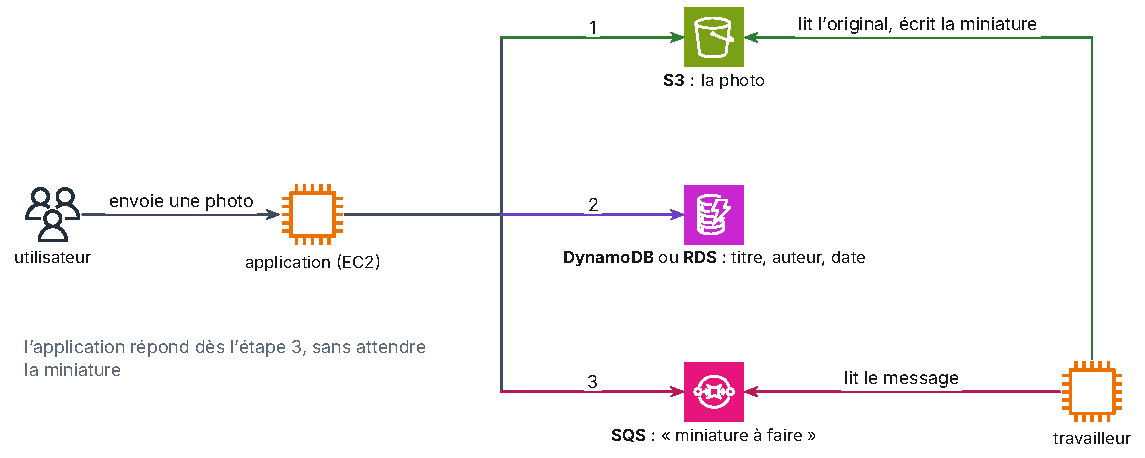
\includegraphics[width=\textwidth]{galerie-evoluee}
    \end{column}
    \begin{column}{.43\textwidth}
      \begin{itemize}
        \setlength{\itemsep}{.5em}
        \item \textbf{S3} : fichiers (images, documents, sauvegardes)
        \item \textbf{RDS} : données structurées, jointures, transactions
        \item \textbf{DynamoDB} : accès par clé à grande échelle, schéma souple
        \item Critères : volume, fréquence d'accès, type de requêtes, cohérence, coût
      \end{itemize}
    \end{column}
  \end{columns}
\end{frame}

% ---- messages -----------------------------------------------------------------
\begin{frame}{Amazon SQS : Simple Queue Service}
  \begin{itemize}
    \setlength{\itemsep}{.45em}
    \item File de messages managée, lancée en 2006
    \item Découple un \textbf{producteur} et un \textbf{consommateur}
    \item Absorbe les pics de charge, tolère l'arrêt d'un consommateur
    \item Opérations : \texttt{SendMessage}, \texttt{ReceiveMessage}, \texttt{DeleteMessage}
    \item Message jusqu'à 1 Mio (256 Kio avant août 2025)
    \item Conservation : 4 jours par défaut, de 1 minute à 14 jours
  \end{itemize}
  \lien{https://docs.aws.amazon.com/AWSSimpleQueueService/latest/SQSDeveloperGuide/welcome.html}
\end{frame}

\begin{frame}{Délai de visibilité}
  \centering
  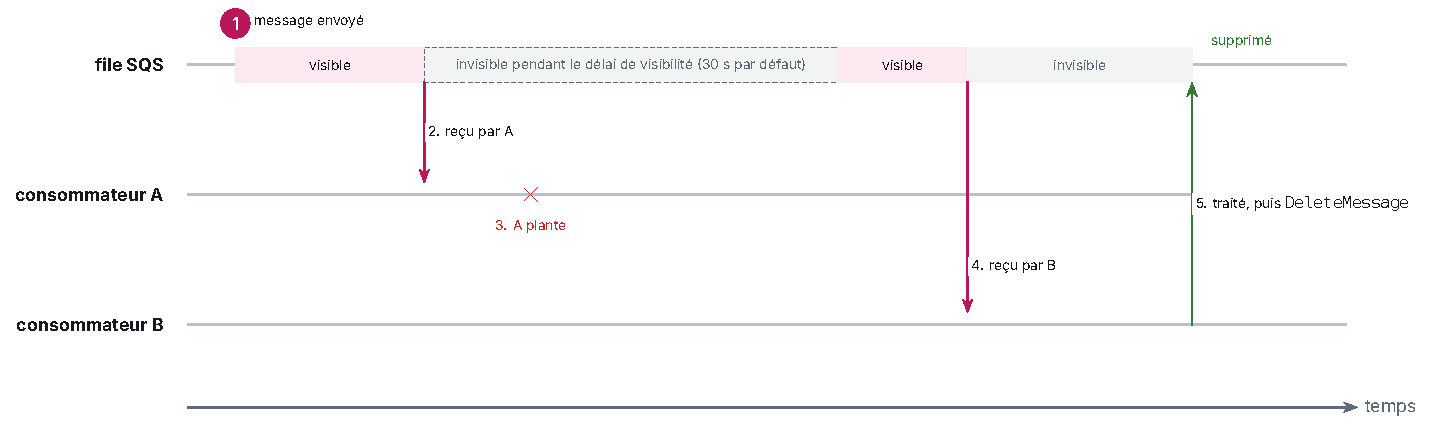
\includegraphics[width=.96\textwidth]{sqs-visibilite}\par\medskip
  \raggedright
  \begin{itemize}
    \item Message reçu = invisible pendant le délai (30 s par défaut, jusqu'à 12 h)
    \item Supprimé seulement par \texttt{DeleteMessage} ; sinon il réapparaît
    \item Conséquence : traitement idempotent côté consommateur
  \end{itemize}
\end{frame}

\begin{frame}{Files standard et FIFO}
  \renewcommand{\arraystretch}{1.4}
  \begin{tabularx}{\textwidth}{@{}>{\raggedright\arraybackslash}p{3.2cm}>{\raggedright\arraybackslash}X>{\raggedright\arraybackslash}X@{}}
    \toprule
    & \textbf{Standard} & \textbf{FIFO} \\ \midrule
    Livraison & au moins une fois & traitement unique \\
    Ordre & au mieux & strict (par groupe de messages) \\
    Débit & quasi illimité & 300 messages/s par action, 3 000 par lots ; plus en mode haut débit \\
    Nom & libre & suffixe \texttt{.fifo} \\ \bottomrule
  \end{tabularx}
  \bigskip
  \begin{itemize}
    \item File de lettres mortes (DLQ) : messages en échec après N réceptions
    \item Attente longue (\emph{long polling}) jusqu'à 20 s : moins de requêtes vides
  \end{itemize}
\end{frame}

\begin{frame}{SQS, SNS, EventBridge}
  \renewcommand{\arraystretch}{1.4}
  \begin{tabularx}{\textwidth}{@{}>{\raggedright\arraybackslash}p{3.2cm}>{\raggedright\arraybackslash}X>{\raggedright\arraybackslash}X@{}}
    \toprule
    \textbf{Service} & \textbf{Modèle} & \textbf{Usage} \\ \midrule
    SQS & file : un message, un consommateur & tâches en arrière-plan, lissage de charge \\
    SNS & publication-abonnement : un message, plusieurs abonnés & notifications, diffusion vers plusieurs files \\
    EventBridge & bus d'événements avec règles de routage & intégration entre services et applications \\ \bottomrule
  \end{tabularx}
  \bigskip
  \begin{itemize}
    \item SQS : premier million de requêtes gratuit chaque mois, puis environ 0,40 \$ par million (standard)
  \end{itemize}
  \source{AWS, \emph{Amazon SQS pricing}.}
\end{frame}

\diapotp{4}{Un bucket, un rôle, une file}{%
  \item Bucket privé, téléversement depuis la console
  \item URL présignée
  \item Instance EC2 avec rôle IAM : lecture et écriture dans S3
  \item File SQS : envoi, réception, délai de visibilité}


% =====================================================================
%  Module 5 : Projet final
% =====================================================================
\section{Projet final}

\begin{frame}{Objectif}
  \begin{itemize}
    \setlength{\itemsep}{.5em}
    \item Déployer une application web publique sur une instance EC2
    \item Fonctions : déposer un fichier (10 Mo au plus), lister les fichiers, les télécharger
    \item Fichiers stockés dans un bucket S3 privé
    \item Application fournie : Flask + boto3 ; travail demandé : le déploiement
  \end{itemize}
  \bigskip
  \textbf{Exigences}
  \begin{itemize}
    \item HTTP (80) et HTTPS (443) ouverts à tous, SSH (22) limité à votre adresse
    \item Aucune clé d'accès sur l'instance : accès à S3 par un rôle IAM
    \item Rôle limité au bucket : lister, lire, écrire, pas de suppression
    \item Redémarrage automatique de l'application (panne, redémarrage de l'instance)
  \end{itemize}
\end{frame}

\begin{frame}{Architecture}
  \centering
  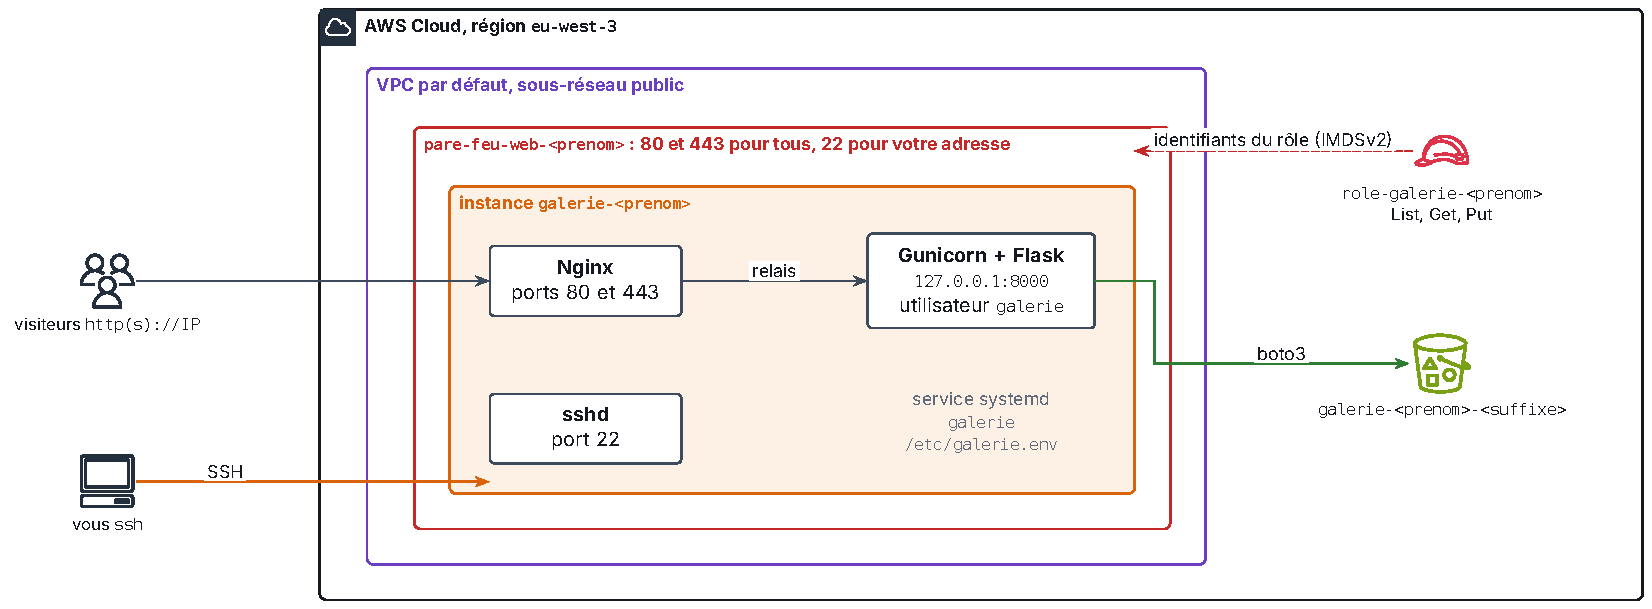
\includegraphics[width=\textwidth]{projet-architecture}
\end{frame}

\begin{frame}{Composants sur l'instance}
  \renewcommand{\arraystretch}{1.4}
  \begin{tabularx}{\textwidth}{@{}>{\raggedright\arraybackslash}p{3.6cm}>{\raggedright\arraybackslash}X@{}}
    \toprule
    \textbf{Nginx} & serveur frontal sur les ports 80 et 443 : TLS, taille maximale des requêtes, relais vers l'application \\
    \textbf{Gunicorn} & serveur d'application Python, 2 processus, écoute sur \texttt{127.0.0.1:8000} uniquement \\
    \textbf{Flask + boto3} & application ; boto3 obtient les identifiants du rôle via IMDSv2 \\
    \textbf{systemd} & service \texttt{galerie} : démarrage au boot, relance en cas d'arrêt \\
    \textbf{Utilisateur \texttt{galerie}} & compte système sans droits d'administration \\
    \textbf{\texttt{/etc/galerie.env}} & configuration : nom du bucket, région ; aucun secret \\ \bottomrule
  \end{tabularx}
\end{frame}

\begin{frame}{Traitement d'une requête}
  \centering
  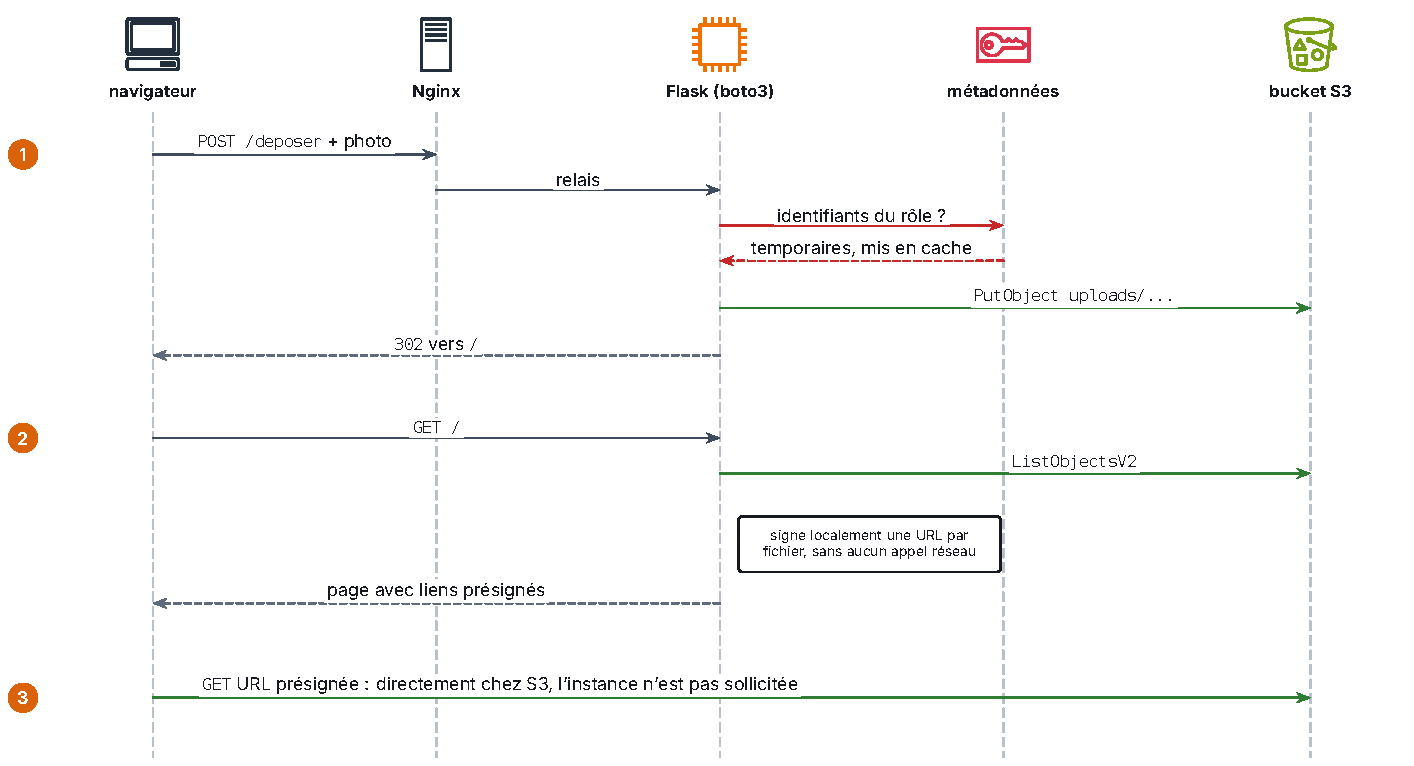
\includegraphics[height=.78\textheight]{projet-requete}
\end{frame}

\begin{frame}{URL présignées}
  \begin{itemize}
    \setlength{\itemsep}{.55em}
    \item URL signée avec les identifiants de l'application, pour un objet et une durée donnés
    \item Générée localement, sans appel réseau
    \item Le navigateur télécharge directement depuis S3 : pas de charge sur l'instance
    \item Durée de validité limitée par celle des identifiants : quelques heures avec un rôle, 7 jours au maximum avec une clé permanente
  \end{itemize}
  \lien{https://docs.aws.amazon.com/AmazonS3/latest/userguide/using-presigned-url.html}
\end{frame}

\begin{frame}{HTTPS}
  \begin{itemize}
    \setlength{\itemsep}{.55em}
    \item Certificat reconnu par les navigateurs : délivré pour un nom de domaine
    \item Projet : certificat autosigné, connexion chiffrée mais avertissement du navigateur
    \item En production :
    \begin{itemize}
      \item nom de domaine (Route 53 ou autre registraire)
      \item certificat gratuit AWS Certificate Manager, sur un répartiteur de charge ou CloudFront
      \item ou certificat Let's Encrypt directement sur Nginx
    \end{itemize}
  \end{itemize}
\end{frame}

\begin{frame}{Vérifications attendues}
  \renewcommand{\arraystretch}{1.15}
  \begin{tabularx}{\textwidth}{@{}>{\raggedright\arraybackslash}p{4.6cm}>{\raggedright\arraybackslash}X@{}}
    \toprule
    \textbf{Exigence} & \textbf{Vérification} \\ \midrule
    Application publique & \texttt{http://IP} et \texttt{https://IP} répondent \\
    SSH restreint & port 22 fermé depuis CloudShell \\
    Application non exposée & port 8000 fermé ; \texttt{ss -ltn} montre \texttt{127.0.0.1:8000} \\
    Bucket privé & URL directe d'un objet : \texttt{AccessDenied} ; URL présignée : accès puis expiration \\
    Aucune clé & pas de \texttt{\textasciitilde/.aws}, aucune clé dans l'application \\
    Moindre privilège & \texttt{aws s3 rm} refusé \\
    Résilience & relance après \texttt{kill -9} et après redémarrage \\ \bottomrule
  \end{tabularx}
\end{frame}

\begin{frame}{Limites et évolutions}
  \begin{columns}[c]
    \begin{column}{.57\textwidth}
      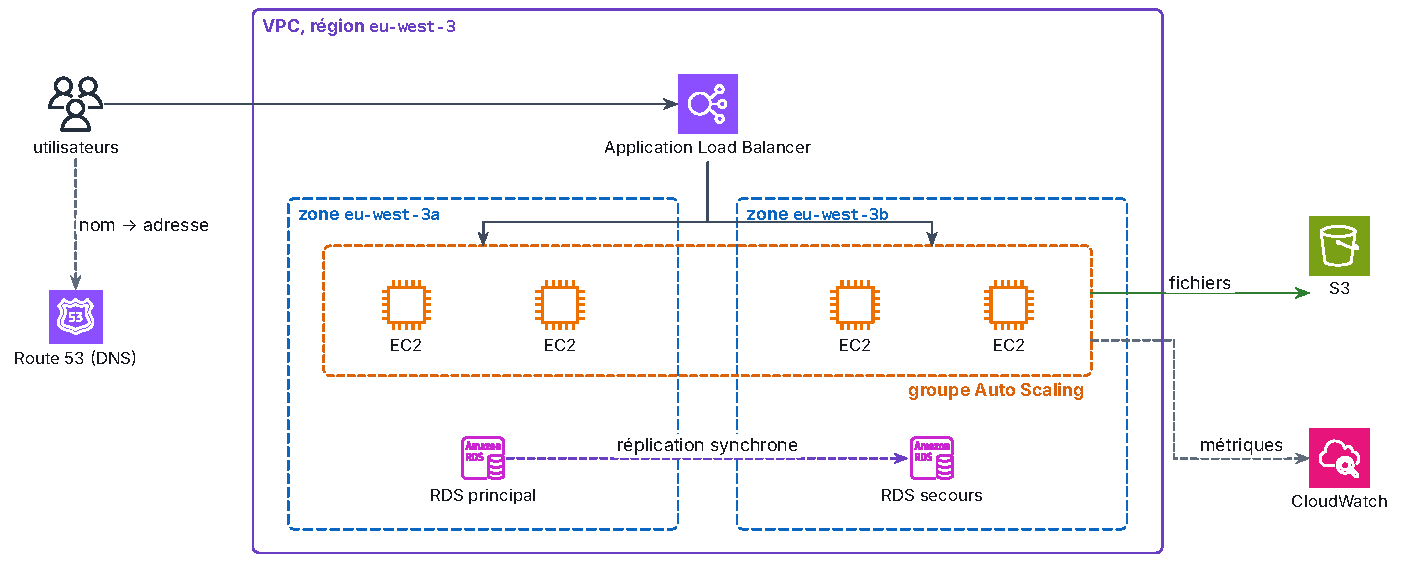
\includegraphics[width=\textwidth]{architecture-cible}
    \end{column}
    \begin{column}{.41\textwidth}
      \begin{itemize}
        \setlength{\itemsep}{.4em}
        \item Une instance, une AZ : pas de haute disponibilité
        \item Adresse IP changeante : nom de domaine, Elastic IP ou répartiteur
        \item Évolutions : ALB + groupe Auto Scaling multi-AZ, RDS Multi-AZ, alarmes CloudWatch
        \item Infrastructure décrite en code : CloudFormation, CDK, Terraform
      \end{itemize}
    \end{column}
  \end{columns}
  \lien{https://docs.aws.amazon.com/wellarchitected/latest/framework/welcome.html}
\end{frame}

\diapotp{5}{Déployer la galerie}{%
  \item Archive de l'application dans le bucket
  \item Instance avec rôle, installation, service systemd
  \item Nginx en HTTP puis en HTTPS
  \item Vérifications, puis suppression de toutes les ressources}


\begin{frame}{Pour aller plus loin}
  \begin{itemize}
    \setlength{\itemsep}{.5em}
    \item Documentation AWS : \url{https://docs.aws.amazon.com}
    \item AWS Well-Architected Framework : six piliers (excellence opérationnelle, sécurité, fiabilité, performance, coûts, durabilité)
    \item AWS Skill Builder : formations et laboratoires en ligne
    \item Certification d'entrée : AWS Certified Cloud Practitioner
    \item Architectures de référence : AWS Solutions Library, \url{https://aws.amazon.com/solutions/}
  \end{itemize}
\end{frame}


\end{document}
